\documentclass[conference]{IEEEtran}
\usepackage{pdfpages, etoolbox, afterpage, graphicx, adjustbox}
\usepackage[hidelinks]{hyperref}


\newcommand\blankpage{%
    \null
    \thispagestyle{empty}%
    \addtocounter{page}{-1}%
    \newpage}

% *** GRAPHICS RELATED PACKAGES ***
%
\ifCLASSINFOpdf
  % \usepackage[pdftex]{graphicx}
  % declare the path(s) where your graphic files are
  % \graphicspath{{../pdf/}{../jpeg/}}
  % and their extensions so you won't have to specify these with
  % every instance of \includegraphics
  % \DeclareGraphicsExtensions{.pdf,.jpeg,.png}
\else
  % or other class option (dvipsone, dvipdf, if not using dvips). graphicx
  % will default to the driver specified in the system graphics.cfg if no
  % driver is specified.
  % \usepackage[dvips]{graphicx}
  % declare the path(s) where your graphic files are
  % \graphicspath{{../eps/}}
  % and their extensions so you won't have to specify these with
  % every instance of \includegraphics
  % \DeclareGraphicsExtensions{.eps}
\fi

\hyphenation{op-tical net-works semi-conduc-tor}


\begin{document}

\title{Malware, when to extract configuration data from system memory}


% author names and affiliations
% use a multiple column layout for up to three different
% affiliations
\author{\IEEEauthorblockN{Jeroen Kraan}
\IEEEauthorblockA{Hogeschool van Amsterdam\\
Email: Jeroen.Kraan@hva.nl}
\and
\IEEEauthorblockN{Ricardo van Zutphen}
\IEEEauthorblockA{Hogeschool van Amsterdam\\
Email: Ricardo.van.Zutphen@hva.nl}}



% make the title area
\maketitle

% As a general rule, do not put math, special symbols or citations
% in the abstract
%\begin{abstract}
%The abstract goes here.
%\end{abstract}

% no keywords




% For peer review papers, you can put extra information on the cover
% page as needed:
% \ifCLASSOPTIONpeerreview
% \begin{center} \bfseries EDICS Category: 3-BBND \end{center}
% \fi
%
% For peerreview papers, this IEEEtran command inserts a page break and
% creates the second title. It will be ignored for other modes.
\IEEEpeerreviewmaketitle


\section{Introduction}
Dynamic malware analysis is an important tool to recognize and help understand new threats in the form of malware. 
Dynamic malware analysis is studying the behaviour of malware while it is being executed on a controlled host computer. This can be in a virtualized environment or on a physical machine. The purpose of dynamic analysis is to collect behavioural data like arguments used in system API calls, the contents of the system memory, and network communications. Network communication is an important way to recognize ‘who’ the malware is communicating with. The ‘who’ is called a command and control server (C2). C2s are part of what is called a malware configuration. This can contain C2s, version numbers, and any other information used by a specific type of malware.\\

One way to collect parts of the configuration data is to look at the network communication of malware. Another type is trying to retrieve the configurations or part of it from process memory dumps.\\

Automated Dynamic malware analysis systems like Cuckoo Sandbox try to automate this process by making memory dumps at a point during the execution of the malware. These memory dumps can then be analysed by various tools. The question is: at what point in execution does the system memory contain the malware configuration?\\

Cuckoo Sandbox is planning to develop a new module to increase the chance of extracting a configuration from the memory. To support this development, this research will be focused on finding the most likely time slot and  possibly  the required events during execution in which the malware configuration will be located in the system memory. 
Our hypothesis: “Creating process memory dumps during the malware execution increases the chance of finding configuration data compared to creating dumps at the end of execution”, will help determine when to create process memory dumps during the malware execution.\\

This research will focus on ransom and banking malware. By ransomware we mean malware that has a focus on extorting a victim by holding hostage of their computer, by encrypting their personal files and asking for a sum of money in order to restore their files. Examples of names of ransomware are: Cryptolocker \cite{tran-cryptolocker}, TeslaCrypt \cite{wyke-currans}, and Locky \cite{long-locky}.
By banking malware, we mean malware that has a focus on stealing financial information, stealing login credentials, keystroke logging, and form manipulation. Examples of names of banking malware are: Dridex \cite{brien-dridex}, Zeus \cite{wyke-zeus}, and Vawtrak \cite{kroustek-vawtrak}. The reason of choosing these types of malware is that the binaries  for this malware are likely to contain configuration data like C2s, because the malware will need to upload the collected data.\\

This paper will be organized as follows:  section 2 will contain a statement of the problem. Section 3 will contain an overview of the collected dataset  used for measurement. Section 4 explains how to recognise the in-memory malware configuration for the collected dataset. Section 5 will contain the result of the measurement. Section 6 will contain the conclusion.\\


\section{Problem statement}

Malware usually communicates with command and control (C2) servers. We call the IP addresses, ports, encryption keys, URLs,   other information used to communicate, and other information used by the malware: configuration data. This data can be embedded in the malware binary, where it is usually encrypted or obfuscated in some way. If malware wants to use the configuration data while being executed on a system, it will need to decrypt the information and load it into the system memory \cite{wyke-confextract}.\\

Dynamic malware analysis systems like Cuckoo Sandbox \cite{cuckoo} can try to take advantage of this. A process memory dump can be made, so that the configuration information can be retrieved from the dump. Cuckoo Sandbox makes these dumps at the end of an analysis. The timing of making this dump is crucial. If the dump is made after a process containing the information has exited, meaning the process has ended and no longer resides in the memory, the information will not be in the dump. This causes Cuckoo analyses to sometimes miss configuration data from malware processes that have already exited.\\

The problem is that the exact moment in time where the information resides in the memory is not usually known. A possible solution for this is using interval-based memory dumping. This approach creates memory dumps at a set interval. The fewer seconds between each interval, the larger the chance of creating a dump containing the desired information. This comes with the drawback of having to search a large amount of memory dumps and possibly ‘just missing’ the right moment to dump \cite{teller-memory}.\\

This research will focus on finding the best moment to create process memory dumps. We will do this by trying to find the most likely moment during the execution of malware in which the configuration data is present in the memory. This information can then be used to implement a more accurate version of the interval-based memory dumping method in Cuckoo Sandbox.\\


\subsection{Research question and goal}
The question this research will try to answer is: 'What is the most likely moment during execution of malware at which the system memory contains the malware configuration data?'\\
\\The hypothesis this research will try to prove is “Creating process memory dumps during the malware execution increases the chance of finding configuration data compared to creating dumps at the end of execution”. What the end of execution is, is determined in the scope section.

The goal is to find a moment during execution in which the configuration data is most likely located in the system memory. This information will be used to develop a new analysis module for the dynamic malware analysis system Cuckoo Sandbox to automatically try to extract malware configurations from memory dumps. The development of this module is not included in this research.

\subsection{Methods}

For this research, ransomware and banking malware will be used. For each type of malware the dataset of samples will consists of two malware families.\\
The samples will be in the form of executable files of the actual malware. This means no malware that will still need to perform some form of exploit to be able to execute will be used.\\\\To analyze these samples, a modified Cuckoo Sandbox instance configured with virtual machines using Windows 7  Professional 64bit as the operating system will be used as the analysis system. \\\\The modified Cuckoo version will support interval-based creation of process memory dumps. The time of the intervals between dumps will be decreased until the configuration data is found in one of the dumps.


\subsection{Virtual machine configuration}

The used hypervisor for the virtual machines for Cuckoo is Virtualbox. The virtual machines will be created by using VMcloak \cite{vmcloak}, an automated virtual machine generation and cloaking tool for Cuckoo Sandbox.\\\\
All virtual machines will have the following specifications:
\begin{itemize}
\item 1 CPU core 3.2 Ghz
\item 2 GB RAM
\item Internet connection
\end{itemize}
\ \\
The installed software on all virtual machines is:
\begin{itemize}
\item Windows 7 Professional 64bit
\begin{itemize}
\item Without any updates, including Service Pack 1
\end{itemize}
\item Adobe PDF reader 9.0
\item Adobe Flashplayer 11.7.700.169
\item Visual studio redistributable packages: 2005 -– 2013.
\item Java JRE 7
\item .NET framework 4.0
\end{itemize}

\ \\Using Yara, a tool using signatures to recognize data structures in binary  data, we will determine if a malware configuration is present in the memory dump or not \cite{roberston-ioc}.

The data collected by measuring the presence of the malware configuration in the memory dumps will be used to create a timeline containing the average time in which the configuration resides in the system memory.


\subsection{Measurement}
To prove or disprove our hypothesis, the time in seconds when the configuration data is in the memory during the execution of the malware, is used. \\\\The system time of the host system of the Cuckoo instance will be used to mark each memory dump with a timestamp. These timestamps will be used to create a timeline of each analysis. On this timeline we can mark where the configuration data was in-memory.\\\\Only dumps created after the moment of infection are used, which is the exact moment the first process has started inside the virtual machine.


\subsection{Scope}
Our hypothesis is that dumping process memory during the execution of malware increases the chance of finding configuration data in the memory dump compared to doing it at the end of the execution. In this research we use Cuckoo Sandbox to run the executables. \\\\This research will only focus on ransomware and banking malware. \\\\For Cuckoo Sandbox a maximum analysis time of 300 seconds will be used. This will be the end of execution. The default Cuckoo Sandbox analysis timeout is 120 seconds. Most processes have exited after this time. As a margin of error, we add another 180 seconds. \\\\The dataset will consist of two types of malware. For each type, a set of samples of two malware families is used. The banking malware families are Zeus and Vawtrak. The ransomware families are Locky and Teslacrypt.


\subsection{Research design}
The research consists out of  multiple steps which are explained below.\\

The first step is the collecting of malware samples of two families for ransomware and banking malware. An external expert malware researcher and Cuckoo Sandbox developer will assist in collecting these. \\\\The current Cuckoo Sandbox version(2.0-RC1) does not support making process memory  dumps at intervals (timeslots). This means a modified version of Cuckoo that does support this will need to be created. This modified version will then be used to create a Cuckoo instance.\\\\Yara, with a set of signatures, will be used to automatically recognize configuration data in the memory. These signatures will be created by first analyzing two samples from each malware family from the dataset using the Cuckoo instance. \\\\The goal of each analysis is to find out when the malware starts communicating with its C2 because at this moment the configuration data should be in the memory.\\The memory dumps created at this moment will be manually analyzed with the goal of finding patterns usable to create Yara signatures.\\\\ When all signatures are ready for usage, all malware samples from the dataset will be executed on the Cuckoo instance. During this execution, all memory dumps are created and sorted per analysis and grouped by family.\\\\For each malware family the Yara signatures will then be used to verify, for each analysis, in which of the memory dumps the configuration data is present. The memory dumps are sorted into timeslots which can later be used in a timeline.\\\\The verification process will be used to conclude in which of the timeslots the configuration data is present. These conclusions will then be used to create a timeline for each analysis.  The timelines of each analysis will then be combined to create a new timeline for the malware family the analyses belong to, showing the average time in which the configuration data is present in memory. These per-family timelines will be combined into one timeline. \\\\This final timeline proves or disproves our hypothesis and should show the most likely moment in which the configuration data is in the memory.\\\\ \textbf{Presentation of results}\\
The measured results will be presented in a visual form by the use of charts and graphs in the form of timelines.


\section{Data Acquisition}

The collected dataset consists of 460 malware samples. The malware families included in this set are Zeus and Vawtrak, which is banking malware, and the families Locky and TeslaCrypt, which are ransomware.  The samples were collected  by first searching for file hashes, which can be used to uniquely identify a file,  and then collecting the corresponding malware samples with the help of an external expert malware researcher. The researcher used his privileges with the online malware analysis platform VirusTotal, to obtain the malware samples. The platforms 'Zeustracker', 'SSL Blacklist', and 'Ransomwaretracker' were used to collect hashes for Zeus, Vawtrak, Locky, and Teslacrypt. These platforms are all part of 'abuse.ch', a platform were malware C2s. binary hashes, and configurations are collected \footnote{\url{https://zeustracker.abuse.ch/faq.php}}. All collected file hashes are listed in appendix A.

\subsection{Attributes}	
This section contains information about each malware family and the collected samples for this family. It lists the amount of samples to be used, the file types in the dataset, and the entropy score for each file. A malware binary can be packed or encrypted in order to hide its code, any configuration data, and any other strings. These are the samples we want to use because they likely contain some form of configuration data. \\\\Compressed and encrypted binaries have a high entropy, this entropy can be measured in the form of Shannon Entropy \cite{hamrock-entropy}. The result of this measurement is a floating point number. Using this number and the table mentioned in \cite{hamrock-entropy}, which contains statistical measures based on different types of data, we can determine if a sample is most likely a native, packed or an encrypted executable.
\\\\

\textbf{Zeus}\\
The hashes for the Zeus samples were collected from 'Zeustracker'\footnote{\url{https://zeustracker.abuse.ch}} and also given to us by the external malware researcher. \\\\The set for this family contains 115 samples, each of these files is either a PE32 or an MS-DOS executable. Zeus is a banking malware family. During execution it will still need to download its configuration file. The URL of the location of this configuration file will be in memory during the execution of samples of this set \cite{wyke-zeus}. The Shannon Entropy score for each sample in the set is 6.578 or higher, the average is 6.936. this indicates that the samples are most likely packed executables \cite{hamrock-entropy}.\\

\textbf{Vawtrak}\\
The hashes for the Vawtrak samples were collected from \cite{sahin-vawtrak} and from 'SSL Blacklist'\footnote{\url{https://sslbl.abuse.ch/}}
\\\\The set for this family contains 115 samples, each of these files is a PE32 executable. Vawtrak is a banking malware family. The binaries in this set do not have to download all their configuration data, part of it is already embedded in the file in the form of  multiple URLS \cite{kroustek-vawtrak}. The Shannon Entropy score for each sample in the set is 6.413 or higher, the average is 7.039. this score lies in between the score of packed and encrypted executables, meaning it could be either \cite{hamrock-entropy}.\\


\textbf{Locky}\\
The hashes for the Locky samples were collected from 'Ransomwaretracker'\footnote{\url{https://ransomwaretracker.abuse.ch/}}  and given to us by the external malware researcher.\\\\The set for this family contains 115 samples, each of these files is a PE32 executable. Locky is a ransomware family. The binaries in this set do not have to download all their configuration data, part of it is already embedded in the file in the form of  multiple URLS \cite{nelson-locky}. The Shannon Entropy score for each sample in this set is 6.367 or higher, the average is 6.999. This score lies in between the score of packed and encrypted executables, meaning it could be either \cite{hamrock-entropy}.\\

\textbf{TeslaCrypt}\\
The hashes for the TeslaCrypt were collected from 'Ransomwaretracker' and given to us by the external malware researcher. \\\\The set for this family contains 115 samples, each of these files is a PE32 executable. TeslaCrypt is a ransomware family. The binaries in this set do not have to download all their configuration data, part of it is already embedded in the file in the form of  multiple URLS \cite{wyke-currans}. The Shannon Entropy score for each sample in this set is 6.068 or higher, the average is 6.777. this indicates that the samples are most likely packed executables, but could also be native executables containing compressed or encrypted sections \cite{hamrock-entropy}.

\section{Recognizing the in-memory malware configuration}
Yara is used to be able to recognize the memory of the processes containing the in-memory malware configurations. To be able to do this, a signature is needed for each malware family. The signatures were created by first using Cuckoo to analyse two or more samples from each family and then finding indicators of compromise(IOC) in the created memory dumps, and collecting IOCs from public sources. \\\\Each signature was tested on a set of 30 analyses of the corresponding malware family. While testing, the possibility of the malware not loading the configuration or the malware process crashing, was taken into account. Therefore the goal was create a signature that matches at least 25 out of 30 cases, before considering the signature usable. \\\\This section will explain what Yara signature will be used to identify the in-memory configuration data for each malware family.\\ All created Yara signatures are listed in appendix B.\\

\textbf{Signature: Zeus}
\\The Zeus Yara signature consists of 18 IOCs in the form of a set of strings. These strings are filenames and are part of a URL stored in the configuration data in the process memory. These recurring strings were found by examining multiple Cuckoo analyses of Zeus and collected from a public source \cite{zeus-ioc}.\\The URLs were found by searching the memory for the resolved domain names by the malware during the Cuckoo analysis. The Zeus signature will match if any of the listed IOCs are found in a memory dump.\\

\textbf{Signature: Vawtrak}
\\The Vawtrak Yara signature consists of 11 IOCs in the form of a set of strings. These strings are filenames and other data that are part of a URL stored in the configuration data in the process memory. These strings were collected by examining multiple Vawtrak Cuckoo analyses and from a public source \cite{vawtrak-ioc}.\\The URLs were found by searching the memory for resolved domain names by the malware during the Cuckoo analysis. The Vawtrak signature will match if any of the listed IOCs are found in a memory dump.\\

\textbf{Signature: Locky}
\\The Locky Yara signature consists of five IOCs: three strings and two byte sequences. Part of this signature was given made available for this research by Jurriaan Bremer, a Cuckoo Sandbox developer and malware researcher. The part of the signature made available is a byte sequence. This byte sequence is the start of the RSA public key structure which Locky uses. The second byte sequence used is part of the instructions file which Locky creates on a user's desktop after the encryption of all files. It serves the purpose to notify a user that their files have been encrypted. The strings are URL fields used by Locky and two strings that are also part of the instructions file.\\All IOCs, except for the RSA structure byte sequence, were collected by examining multiple Locky Cuckoo analyses and from a public source \cite{nelson-locky}. The Locky signature will match if any of the IOCs are found in a memory dump.\\

\textbf{Signature: Teslacrypt}
\\The Teslacrypt Yara signature consists of three IOCs: one byte sequence and two strings. One string is part of the instructions file which Teslacrypt creates to notify the user their files have been encrypted. The second string is part of a TOR Network URL which is presented to the user to pay the ransom and restore their files. The byte sequence consists of URL form fields with wildcards between them. These wildcards were used so that the signature would still match if the form fields contain any data.\\All IOCs used in this signature were found by examining multiple Teslacrypt Cuckoo analyses. The Teslacrypt signature will match if any of the IOCs are found in a memory dump.\\


\section{Analysis results}
This section contains the per-family results of the measurement performed process memory dumps created during Cuckoo Sandbox analyses with a length of 300 seconds. Two types of malware were used: Banking malware and Ransomware.  For these types the families Zeus, Vawtrak (Banking malware), Teslacrypt, and Locky (Ransomware) were used.\\\\ The analysis results a grouped into different types of behavior. For each of these groups a possible reason is given which explains why the results are what was measured. During the examination of the measured results, multiple types of behavior were found. These different types of behavior are the cause for the differences in the amount of in-memory configurations found at a certain time interval. The types of behavior are grouped together for each family. Each of these groups is briefly explained and a corresponding timeline for that group is shown. \\The behavior of groups that is not expected will also be briefly explained and can be found at the end of this chapter. Mind that these explanations are hypotheses, further research into the behavior is recommended to draw a proper conclusion about why this behavior occurs.


\subsection{Results Zeus}
The analysis of the Zeus family resulted in data for 104 out of 115 used malware samples. 11 of the samples crashed upon execution. These samples are not part of any timelines or charts discussed in this subsection. Figure \ref{fig:zeus-bar} shows the presence of configuration data for all measured Zeus analyses. This chart was created by combining the timelines for all Zeus analyses. All seperate timelines can be found at \footnote{\url{https://oege.ie.hva.nl/~zutpher003/research2016/zeus/}}.\\

\begin{figure}[!h]
	\hspace{-3cm}
    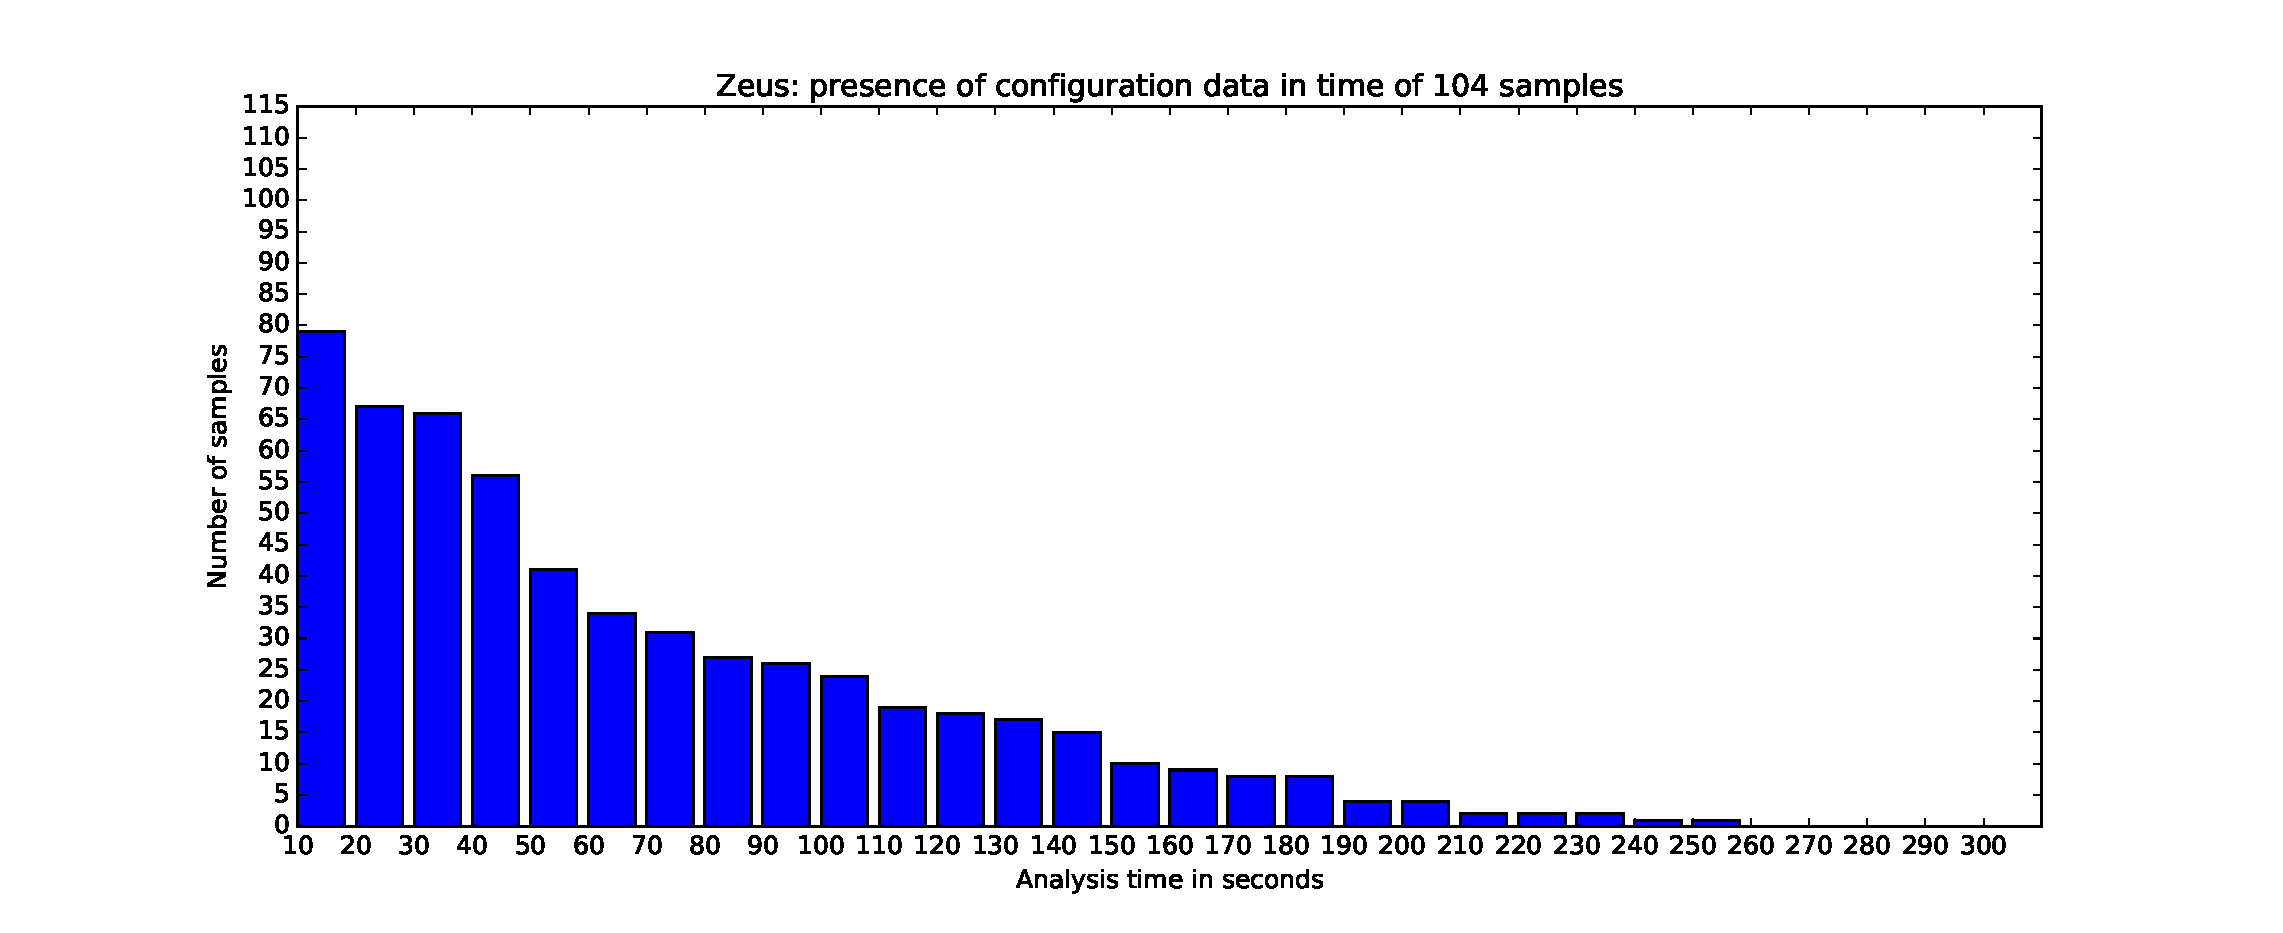
\includegraphics[width=13cm,trim=-95mm 0mm 0mm 9mm, clip=true]{images/zeus/Zeus-barchart.eps}
    \caption{A chart showing the combined timelines of presence of configuration data during the analysis of all Zeus samples}
    \label{fig:zeus-bar}
\end{figure}

\newpage
\textbf{Expected Zeus behavior}
\\Analyses in this group display the expected Zeus behavior: \cite{wyke-zeus} after execution of the first binary, its process creates a copy of itself to a second binary. The first process then starts a second process using the copied binary and writes to its process memory, after which, the first process terminates.\\ Shortly after the second process has started, it starts to unpack a third binary file by to reading it from its own binary. As soon as this is done, a process is started using the third binary.
\\\\The third binary is the actual Zeus malware which performs the malicious actions. It is possible that this third binary also copied itself and creates a process of this copy, but this is not always the case. Before trying to perform a range of different malicious actions (collecting passwords, editing settings etc), the malicious process tries to contact its C2. After this step, a batch script is created which deletes all previous binary files used to infect the system. Up until this moment, the configuration data included in the binary, is found in the memory. The process of copying, unpacking, contacting the C2, and erasing the binaries used to infect the system takes from 10 to 100 seconds. This is also the time the configuration data is present in the memory. The average is 40 seconds.  Figure \ref{fig:zeus-timeline-normal} is a corresponding timeline for this group. \\\\A second type of behavior is included in this group. It is similar to the type mentioned above. The difference is that this type does not start by copying itself, but by first delaying execution time by making the first process 'sleep'. After the sleep, normal execution resumes. The average time of when the configuration data is in memory is from 70 to 130 seconds. Figure \ref{fig:zeus-timeline-normal-delay} shows a timeline of an analysis of this type.


\newpage

\textbf{Explorer.exe injection}
\\After the first process executes, it does not create a copy of itself and starts to unpack a second binary by reading it from its own binary file. The unpacked binary injects itself into another process by acquiring a process handle for the Windows process Explorer.exe, and writes to the memory of this process. The configuration data is present in the memory of this process, but is not visibly used. The configuration data then reamins in the explorer.exe process for an average time of 240 seconds. Figure \ref{fig:zeus-timeline-injection} shows a timeline for an analysis of this group.\\

\textbf{Idle or failed}
\\This group includes two types of analyses: analyses that crash during execution and ones that execute only the first process and then delay the execution until the end of the analysis. For both of these type, the configuration data is not present in the memory. Figure \ref{fig:zeus-timeline-idle} shows a timeline of an analysis of this type.


\begin{figure}[h]
    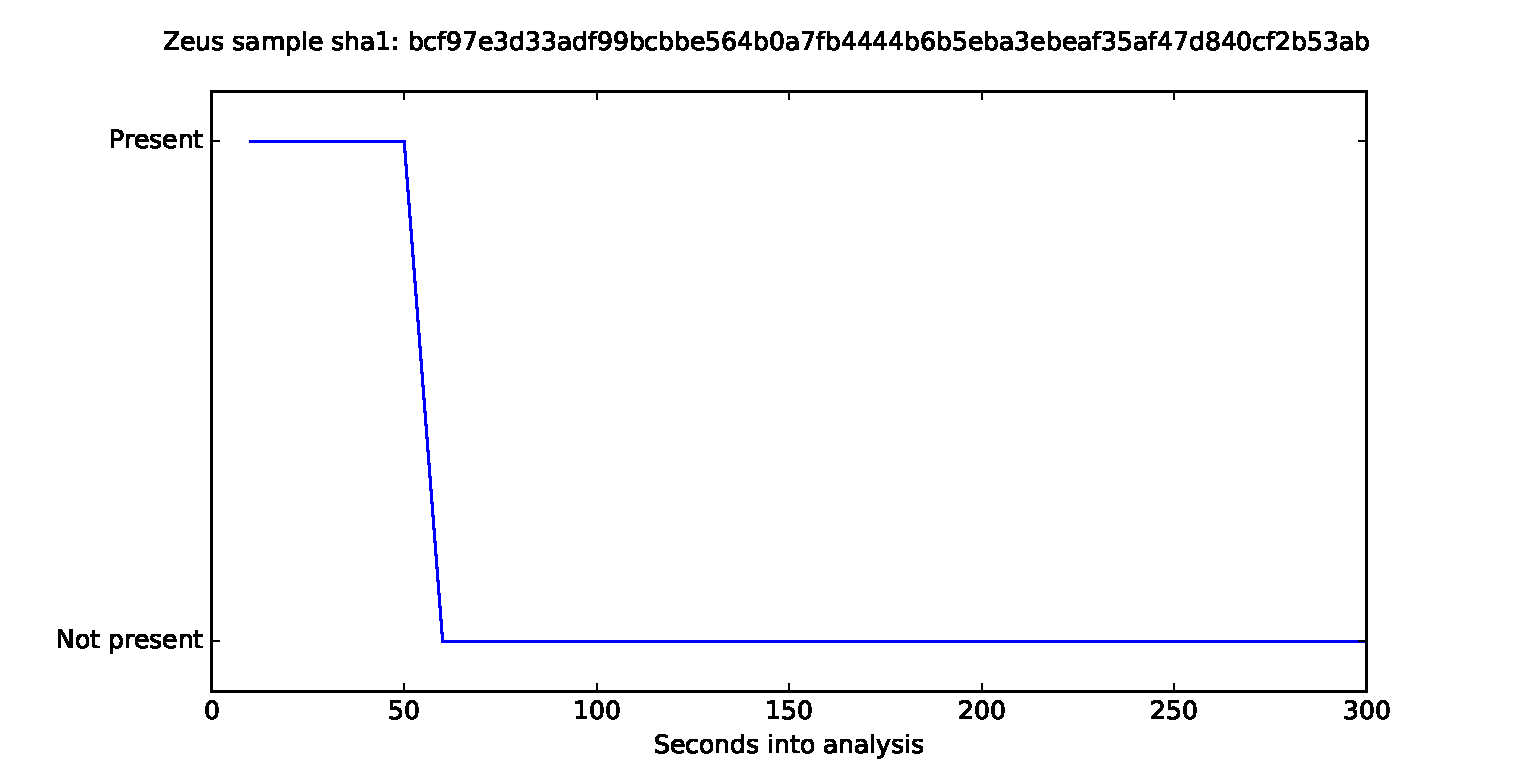
\includegraphics[width=8cm,scale=0.5]{images/zeus/zeus-timelines-eps/Zeus-bcf97e3d33adf99bcbbe564b0a7fb4444b6b5eba3ebeaf35af47d840cf2b53ab.eps}
    \caption{A Zeus timeline showing the average of in-memory configuration data for an analysis in the 'Expected' group}
    \label{fig:zeus-timeline-normal}
\end{figure}
\begin{figure}[h]
    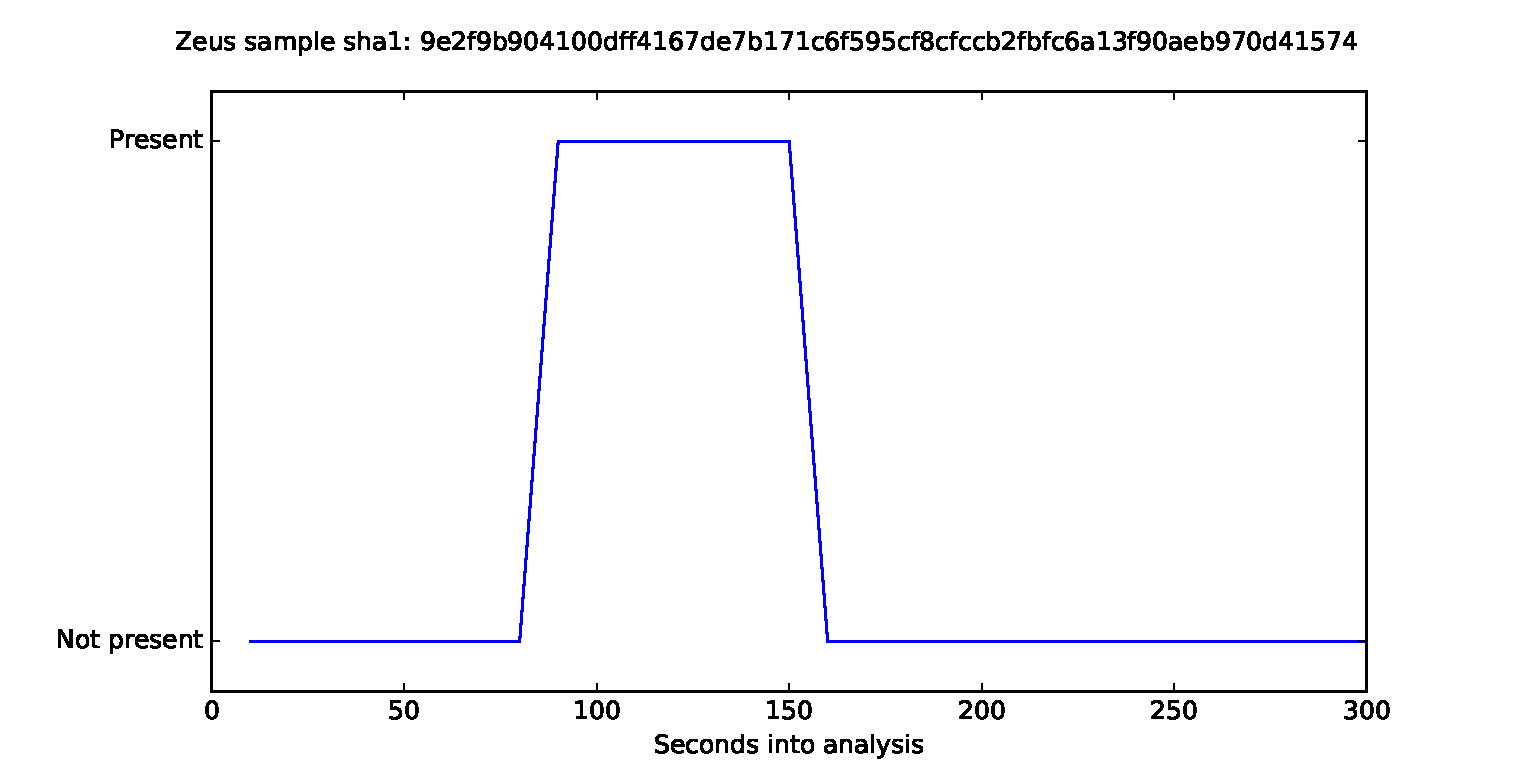
\includegraphics[width=8cm,scale=0.5]{images/zeus/zeus-timelines-eps/Zeus-9e2f9b904100dff4167de7b171c6f595cf8cfccb2fbfc6a13f90aeb970d41574.eps}
    \caption{A Zeus timeline showing the average of in-memory configuration data for an analysis the 'Expected' group, but with a delay in execution at the start}
    \label{fig:zeus-timeline-normal-delay}
\end{figure}
\begin{figure}[h]
    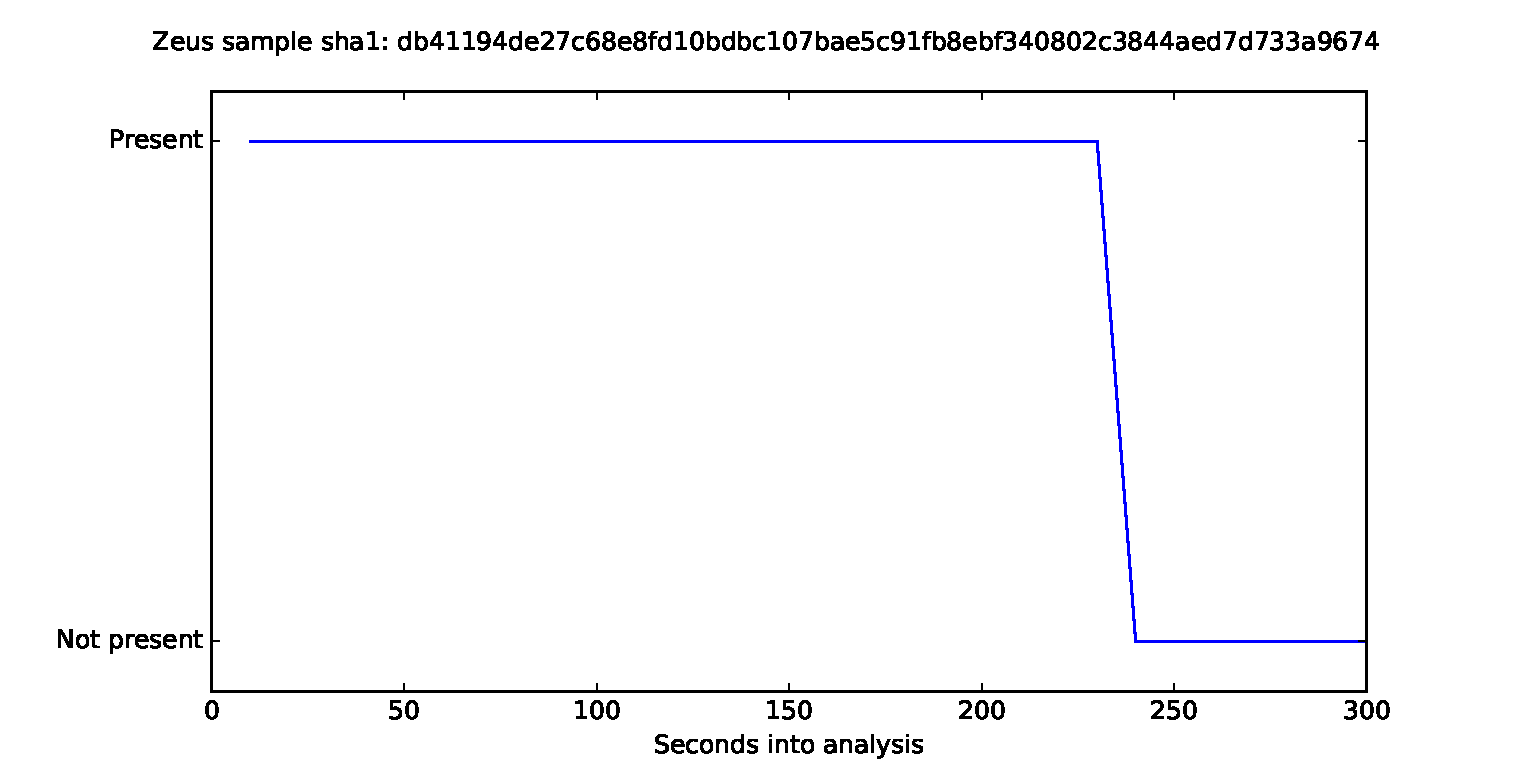
\includegraphics[width=8cm,scale=0.5]{images/zeus/zeus-timelines-eps/Zeus-db41194de27c68e8fd10bdbc107bae5c91fb8ebf340802c3844aed7d733a9674.eps}
    \caption{A Zeus timeline showing the average of in-memory configuration data for an analysis in the
    'Explorer.exe injection' group}
    \label{fig:zeus-timeline-injection}
\end{figure}
\begin{figure}[!h]
    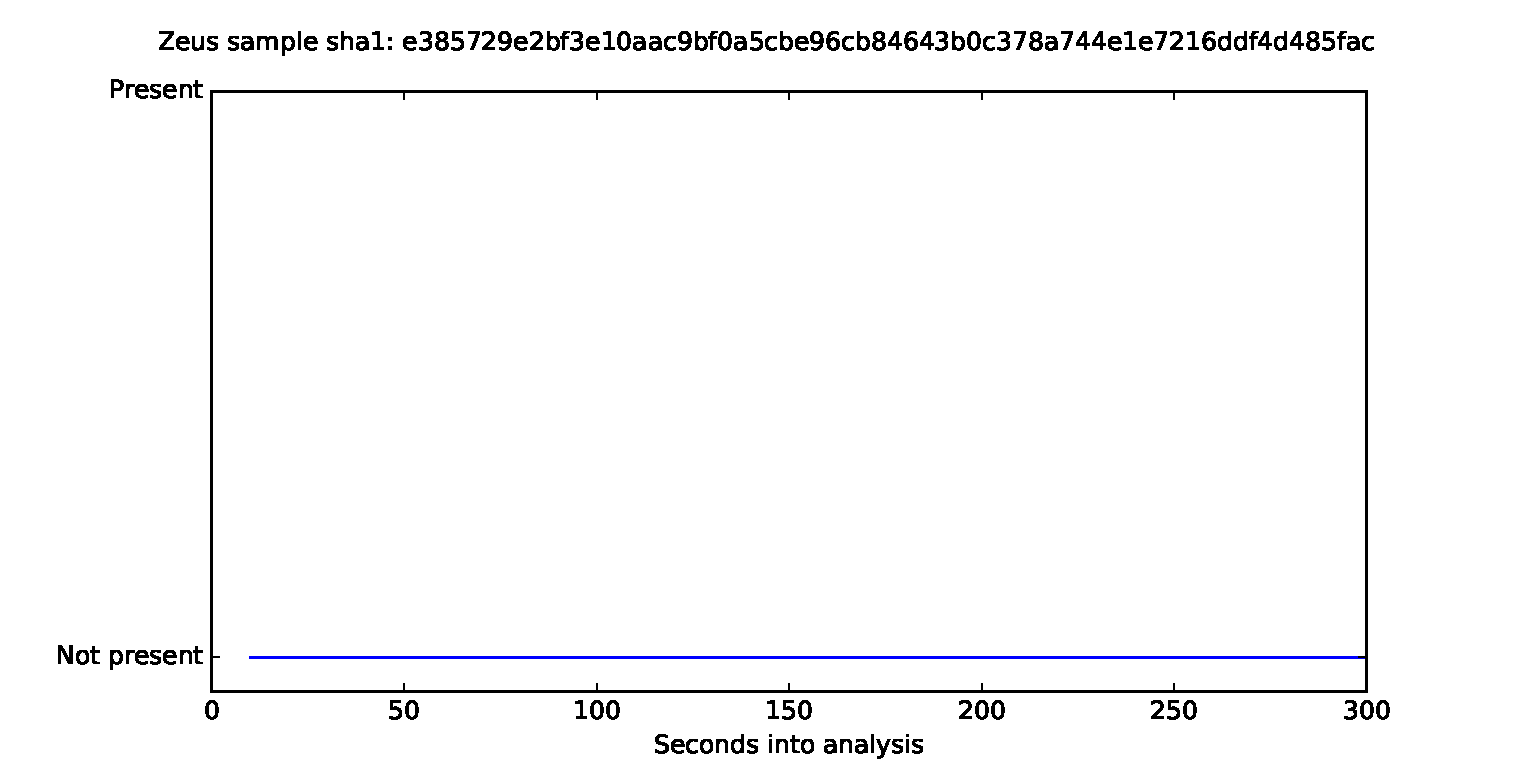
\includegraphics[width=8cm,scale=0.5]{images/zeus/zeus-timelines-eps/Zeus-e385729e2bf3e10aac9bf0a5cbe96cb84643b0c378a744e1e7216ddf4d485fac.eps}
    \caption{A Zeus timeline showing the average of in-memory configuration data for the 'Idle or failed' group}
    \label{fig:zeus-timeline-idle}
\end{figure}

\newpage

\subsection{Results Vawtrak}
The analysis of the Vawtrak family resulted in data for 107 out of 115 used malware samples. 8 of the samples crashed upon execution. These samples are not part of any timelines or charts discussed in this subsection. Figure \ref{fig:vawtrak-bar} shows the presence of configuration data for all measures Vawtrak analyses. This chart was created by combining the timelines for all Vawtrak analyses. All seperate timelines can be found at \footnote{\url{https://oege.ie.hva.nl/~zutpher003/research2016/vawtrak/}}.


\begin{figure}[h]
	\hspace{-3cm}
    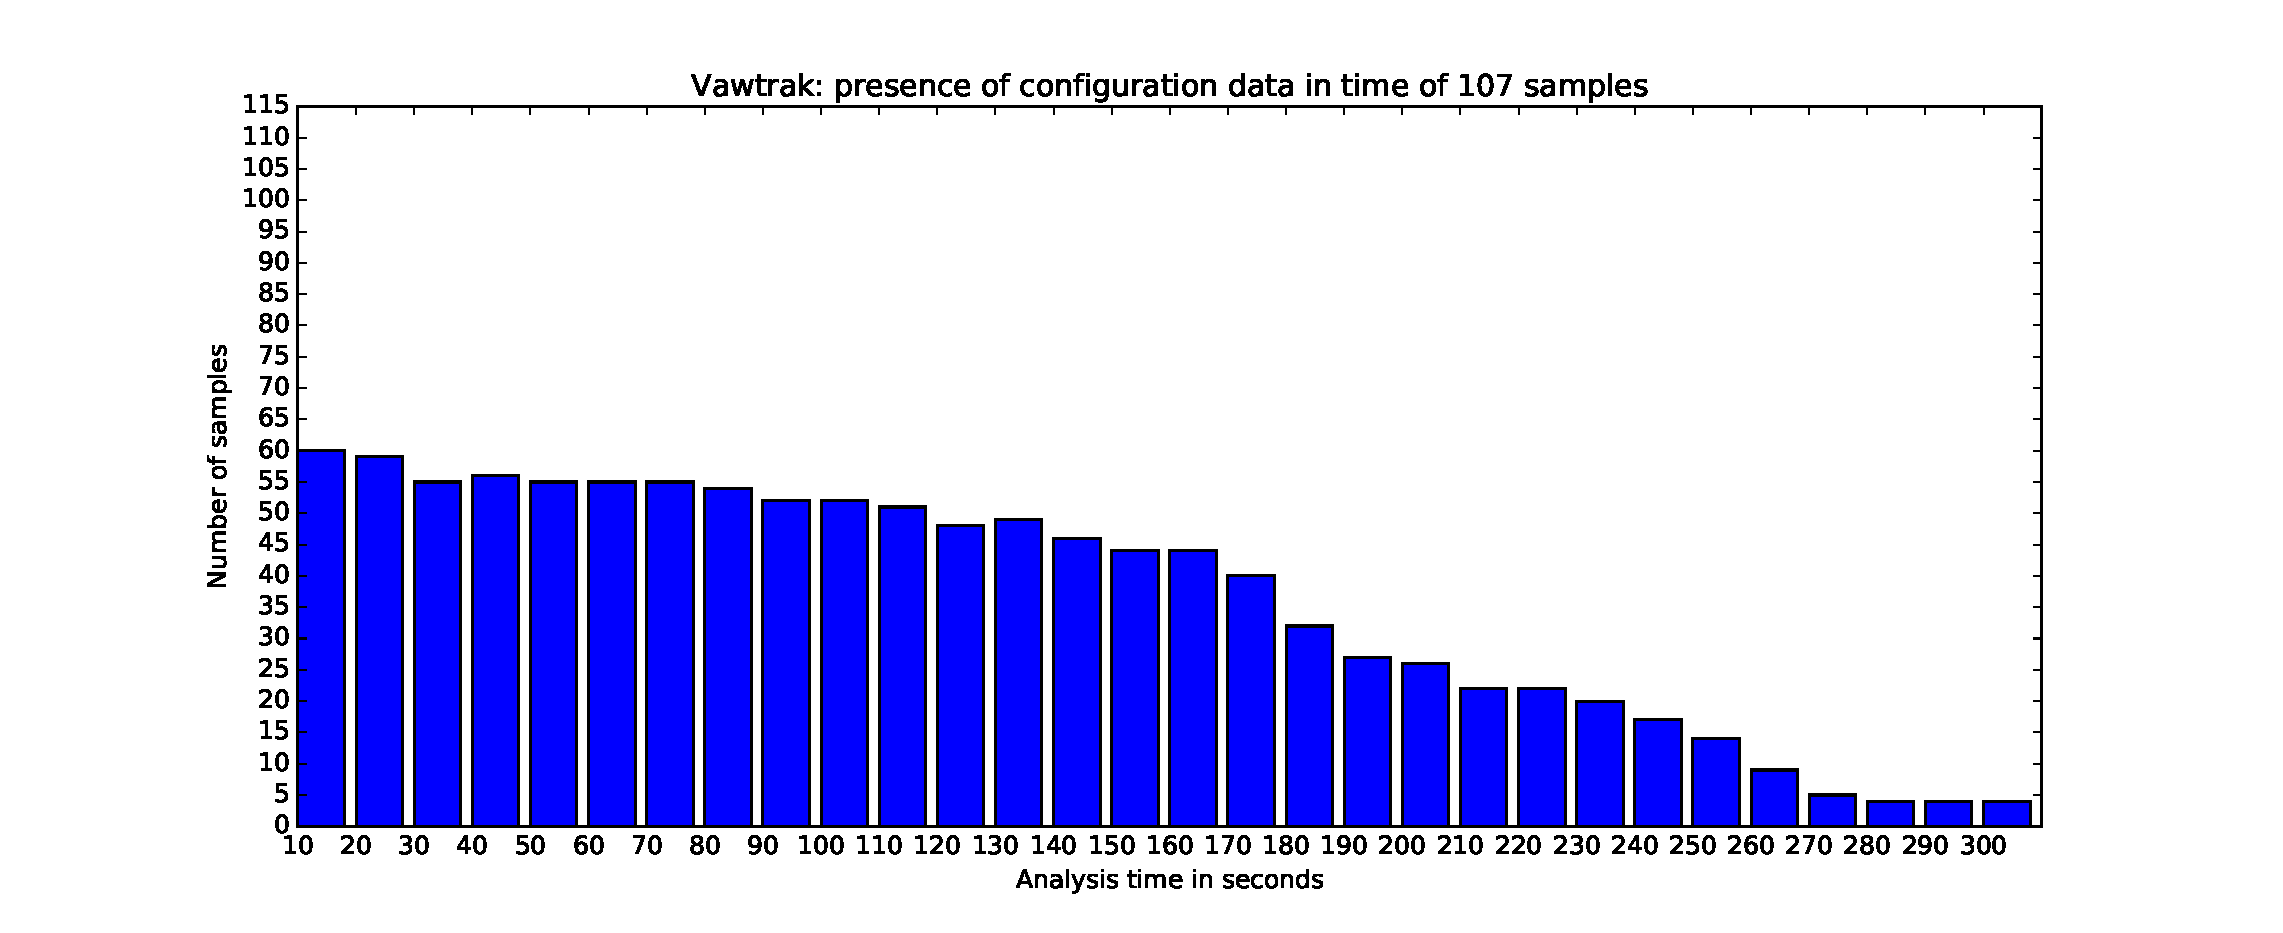
\includegraphics[width=13cm,trim=-70mm 0mm 0mm 9mm, clip=true]{images/vawtrak/Vawtrak-barchart.eps}
    \caption{A chart showing the combined timelines of presence of configuration data during the analysis of all Vawtrak samples}
    \label{fig:vawtrak-bar}
\end{figure}

\newpage

\textbf{Expected Vawtrak behavior}
\\Analyses in this group are of multiple types, they all display the expected Vawtrak behavior \cite{kroustek-vawtrak}, but with slight differences that are noticable in the timeline. \\After the execution of the binary, the process starts by looking for registry keys and file paths of commonly used software and tries to find stored credentials. At this point, the configuration data is in the memory. The next step taken differs per type of analysis: some start a one to two minute execution delay by making the process sleep, and after the delay try to contact its C2. The other type does not delay the execution and  tries to communicate with its C2 immediately after the step of collecting credentials.\\ Timelines for this group show that the configuration data is present in the memory 10 to 200 after the analysis has started. Figure \ref{fig:vawtrak-timeline-normal} shows a timeline for an analysis of this group.\\


\textbf{Brief Vawtrak behavior}
\\Analyses in this group do display Vawtrak behavior\cite{kroustek-vawtrak}, but only briefly. After the execution of its binary, the process starts by looking for registry keys and file paths of commonly used software and tries to find stored credentials. The process does not try to contact its C2. The next step taken is creating a Windows batch file containing code to delete the Vawtrak binary and itself. This file is then executed. Timelines for this group of analyses show that the configuration data is present in the memory for 10 to 30 seconds after the analysis has started. Figure \ref{fig:vawtrak-timeline-brief} shows a timeline for an analysis of this group.\\

\textbf{Injection into other process}
\\Analyses in this group start by delaying execution by sleeping for one to two minutes, during which the configuration data is not present in the memory. After the delay, the process starts unpacking a second binary from its own binary. At this time, the configuration data is present in the memory. When the process has finished unpacking the second binary, it configures Windows to start the binary at Windows startup. The last step taken is injecting itself into another process by acquiring a process handle and writing to its memory. The Windows process being injected seems to be different every analysis. Figure \ref{fig:vawtrak-timeline-injection} shows a timeline for an analysis of this group.\\

\textbf{Idle}
\\Analyses in this group do not have any configuration data in the memory at any point during the analysis. The started process delays the analysis by sleeping immediately after  being executed. These sleeps last for one to three minutes, after which it injects itself into another process by acquiring a process handle and writing to its memory. Figure \ref{fig:vawtrak-timeline-idle} shows a timeline for an analysis of this group.
\newpage

\begin{figure}[h]
    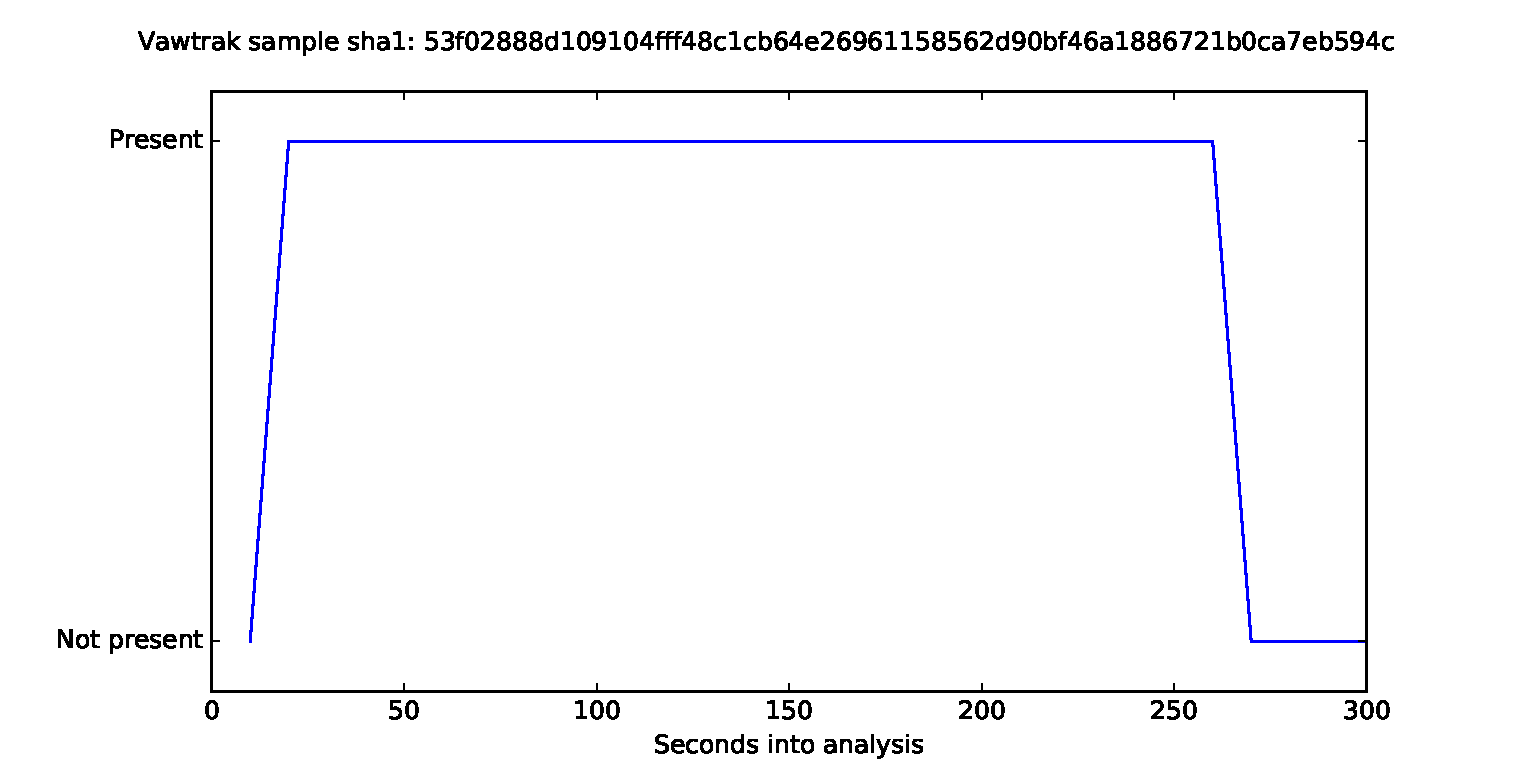
\includegraphics[width=8cm,scale=0.5]{images/vawtrak/vawtrak-timelines-eps/Vawtrak-53f02888d109104fff48c1cb64e26961158562d90bf46a1886721b0ca7eb594c.eps}
    \caption{A Vawtrak timeline showing the average of in-memory configuration data for an analysis in the 'Expected' group}
    \label{fig:vawtrak-timeline-normal}
\end{figure}
\begin{figure}[h]
    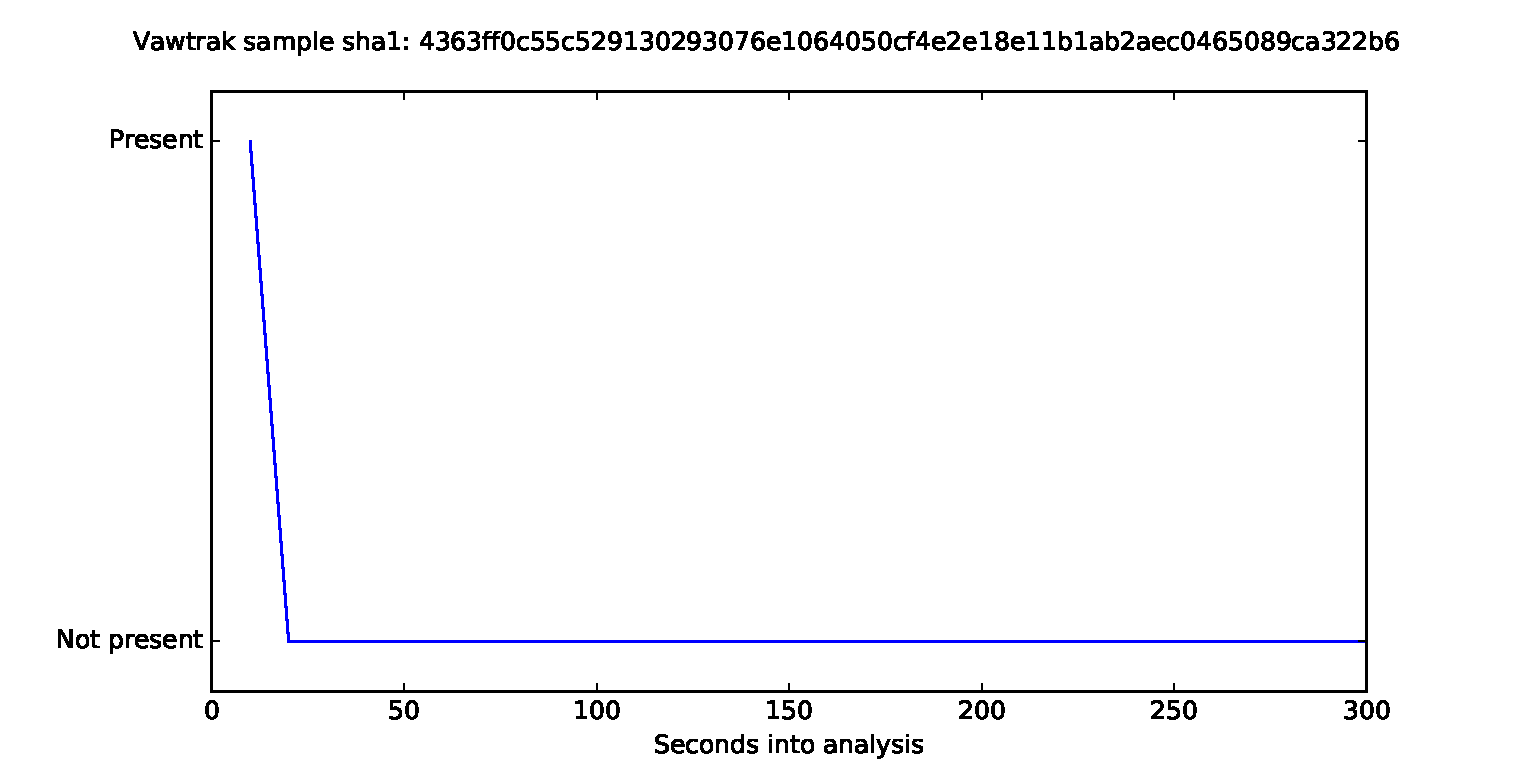
\includegraphics[width=8cm,scale=0.5]{images/vawtrak/vawtrak-timelines-eps/Vawtrak-4363ff0c55c529130293076e1064050cf4e2e18e11b1ab2aec0465089ca322b6.eps}
    \caption{A Vawtrak timeline showing the average of in-memory configuration data for an analysis the 'Brief' group}
    \label{fig:vawtrak-timeline-brief}
\end{figure}
\begin{figure}[!h]
    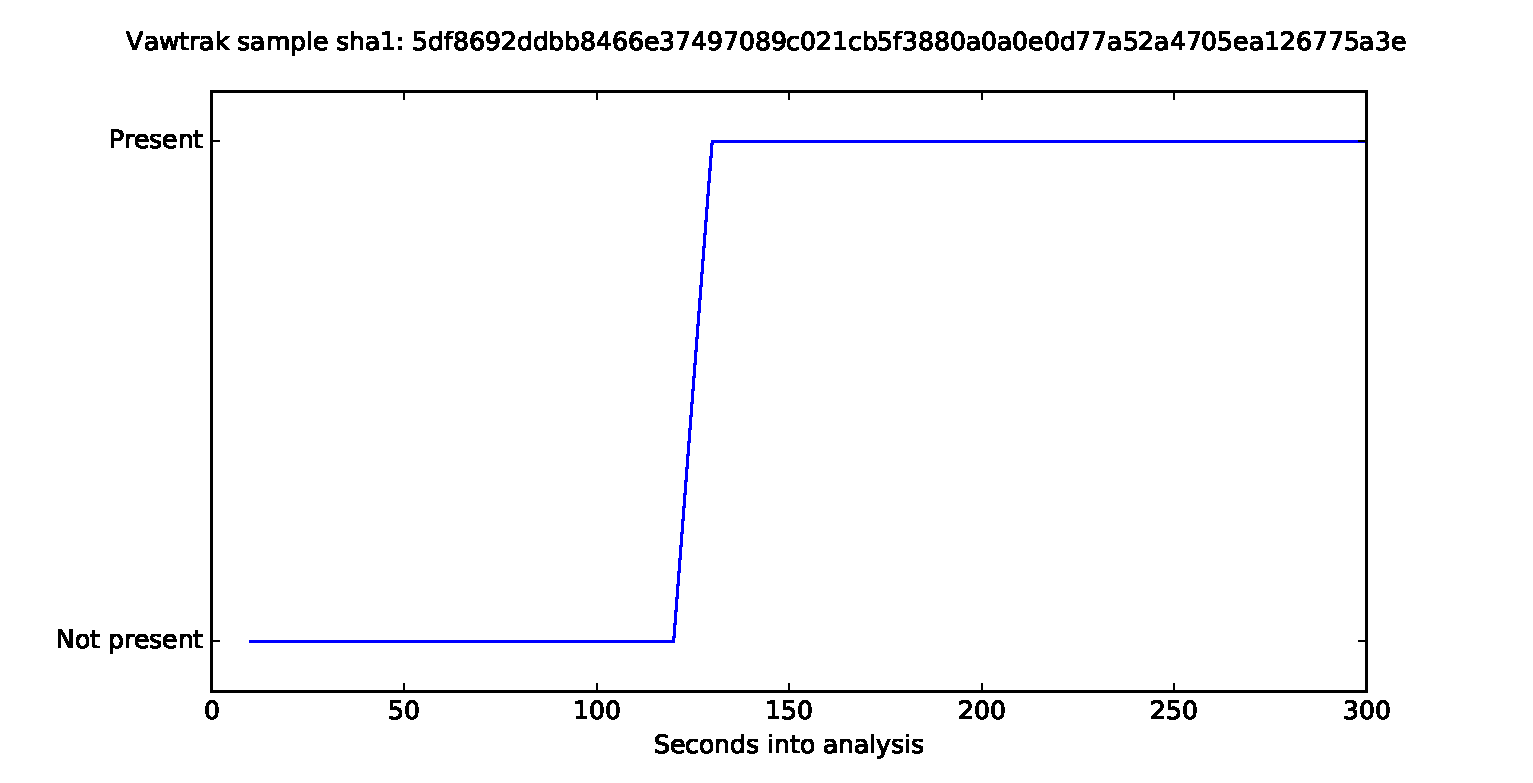
\includegraphics[width=8cm,scale=0.5]{images/vawtrak/vawtrak-timelines-eps/Vawtrak-5df8692ddbb8466e37497089c021cb5f3880a0a0e0d77a52a4705ea126775a3e.eps}
    \caption{A Vawtrak timeline showing the average of in-memory configuration data for an analysis in the 'Other process injection' group}
    \label{fig:vawtrak-timeline-injection}
\end{figure}
\begin{figure}[!h]
    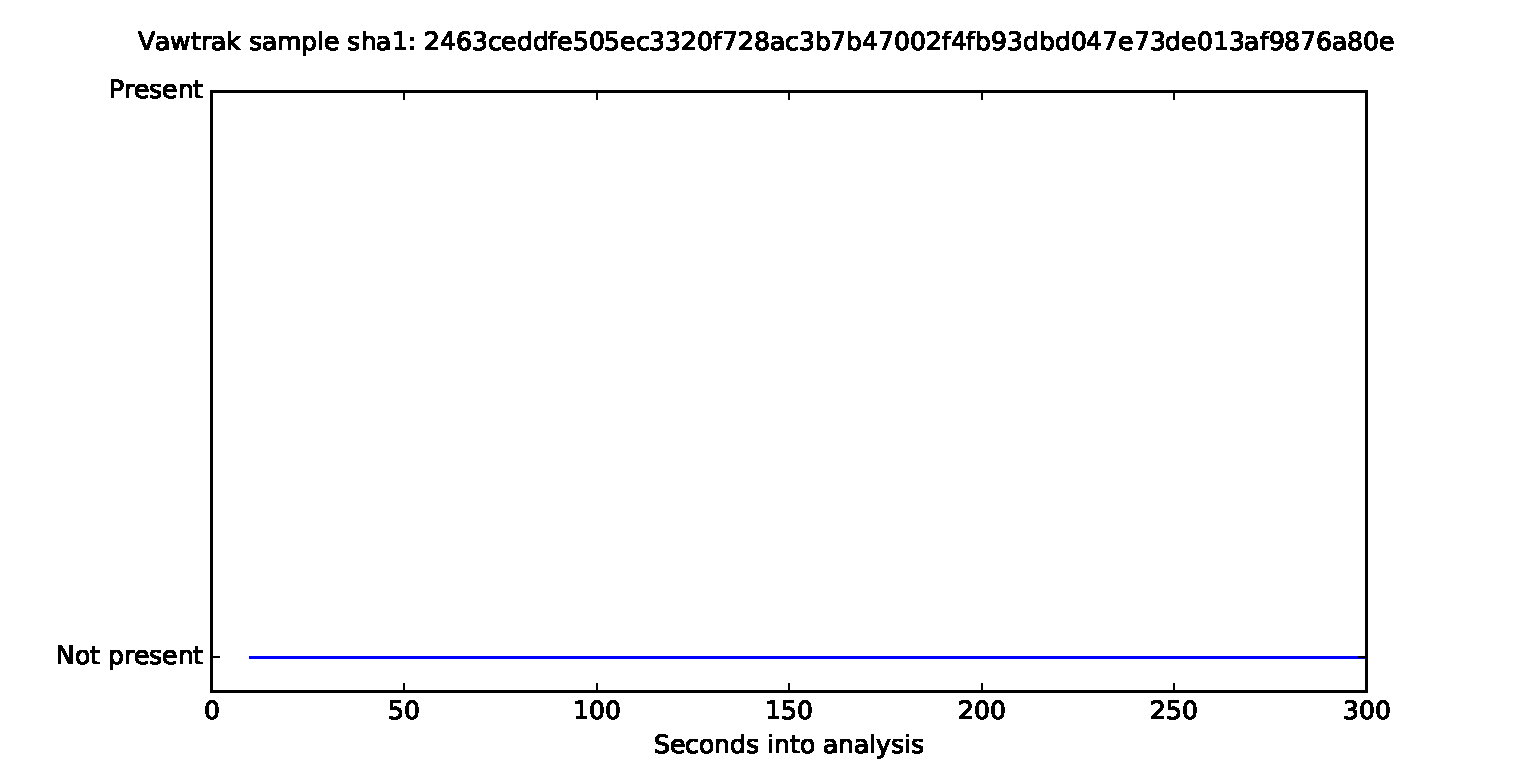
\includegraphics[width=8cm,scale=0.5]{images/vawtrak/vawtrak-timelines-eps/Vawtrak-2463ceddfe505ec3320f728ac3b7b47002f4fb93dbd047e73de013af9876a80e.eps}
    \caption{A Vawtrak timeline showing the average of in-memory configuration data for the 'Idle' group}
    \label{fig:vawtrak-timeline-idle}
\end{figure}


\subsection{Results Locky}
The analysis of the Locky family resulted in data for 114 out of 115 used malware samples. one of the samples crashed upon execution. This sample is not part of any timelines or charts discussed in this subsection. Figure \ref{fig:locky-bar} shows the presence of configuration data for all measured Locky analyses. This chart was created by combining the timelines for all Locky analyses. All seperate timelines can be found at \footnote{\url{https://oege.ie.hva.nl/~zutpher003/research2016/locky/}}.\\


\begin{figure}[h]
	\hspace{-3cm}
    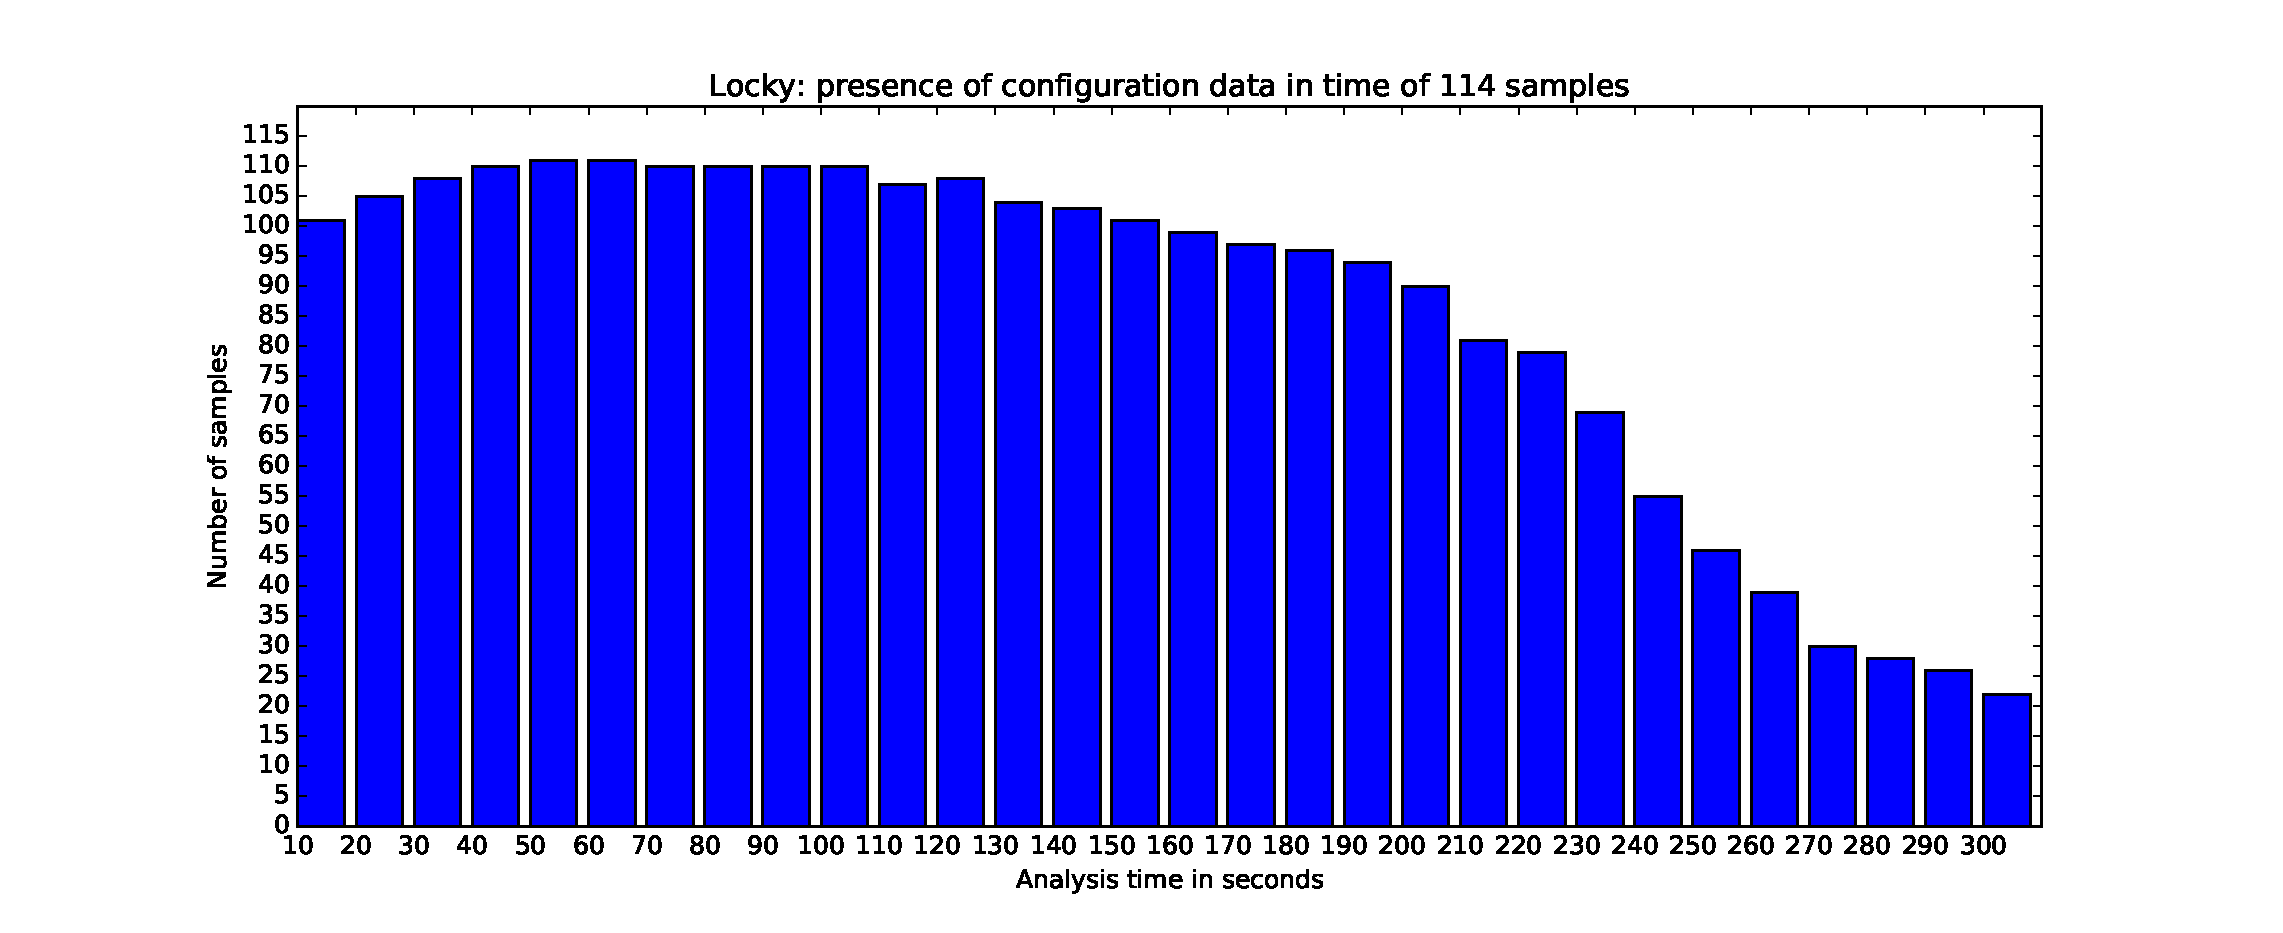
\includegraphics[width=13cm,trim=-70mm 0mm 0mm 9mm, clip=true]{images/locky/Locky-barchart.eps}
    \caption{A chart showing the combined timelines of presence of configuration data during the analysis of all Locky samples}
    \label{fig:locky-bar}
\end{figure}


\textbf{Expected Locky behavior}
\\Analyses in this group display the 'expected' Locky behavior \cite{nelson-locky}: The first process of the Locky malware starts with trying to communicate with the C2. After this moment there are two types of behaviour in the analyses. The case where the C2 responds, Locky will now start encrypting files on the computer and after the encryption a second process is started which deletes all Windows shadow copies. The last step performed is creating a notification to inform the user that their files have been encrypted.\\

The second type of behaviour is where the C2 does not respond. In this case, the process will try to contact the other C2s in memory, and if these do not respond, the process will terminate. For both these cases the configuration data is in-memory from start of the analysis until the first process terminates.\\

The timelines for this group of analyses show that the configuration data is present in the memory for 10 to 290 seconds after the analysis has started.\\

Figure \ref{fig:locky-timeline-expected} shows a timeline for an analysis of this group.\\

\textbf{Continuous communication }\\
Analyses in this group immediately start to communicate with their C2, which is not responding, and continue to do so until the end of the analysis. The configuration data is present in the memory during the entire length of the analysis. This corresponds with the expected behavior of some of the analyzed Locky samples in \cite{nelson-locky}.

Figure \ref{fig:locky-timeline-continuous} shows a timeline for an analysis of this group.\\
 
\textbf{Idle}\\
Analyses in this group start to delay the execution after being started by making the process sleep. The memory does not contain any configuration data during the length of these analyses.

Figure \ref{fig:locky-timeline-idle} shows a timeline for an analysis of this group.\\


\begin{figure}[h]
    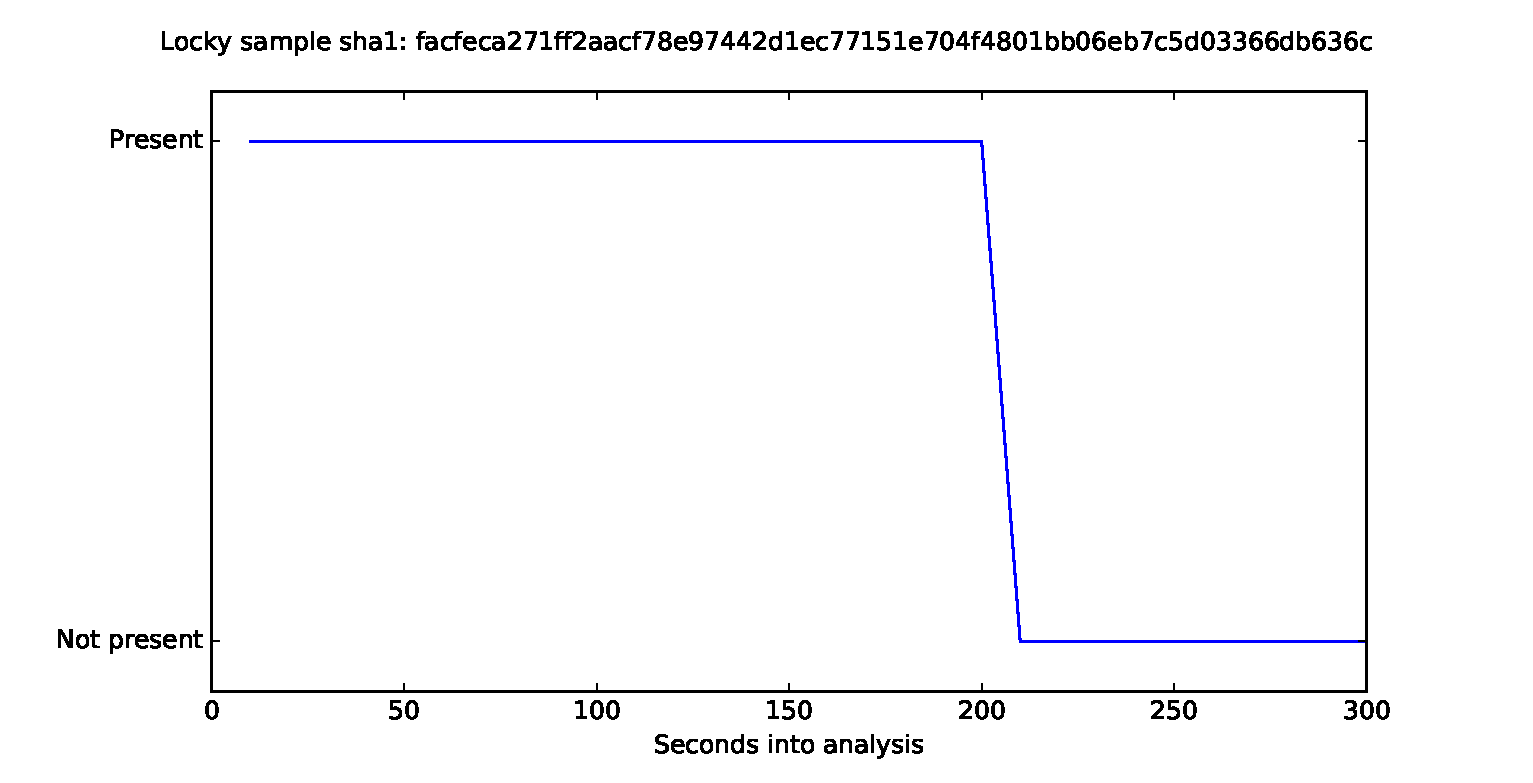
\includegraphics[width=8cm,scale=0.5]{images/locky/locky-timelines-eps/Locky-facfeca271ff2aacf78e97442d1ec77151e704f4801bb06eb7c5d03366db636c.eps}
    \caption{A Locky timeline showing the average of in-memory configuration data for an analysis the 'Expected' group}
    \label{fig:locky-timeline-expected}
\end{figure}
\begin{figure}[!h]
    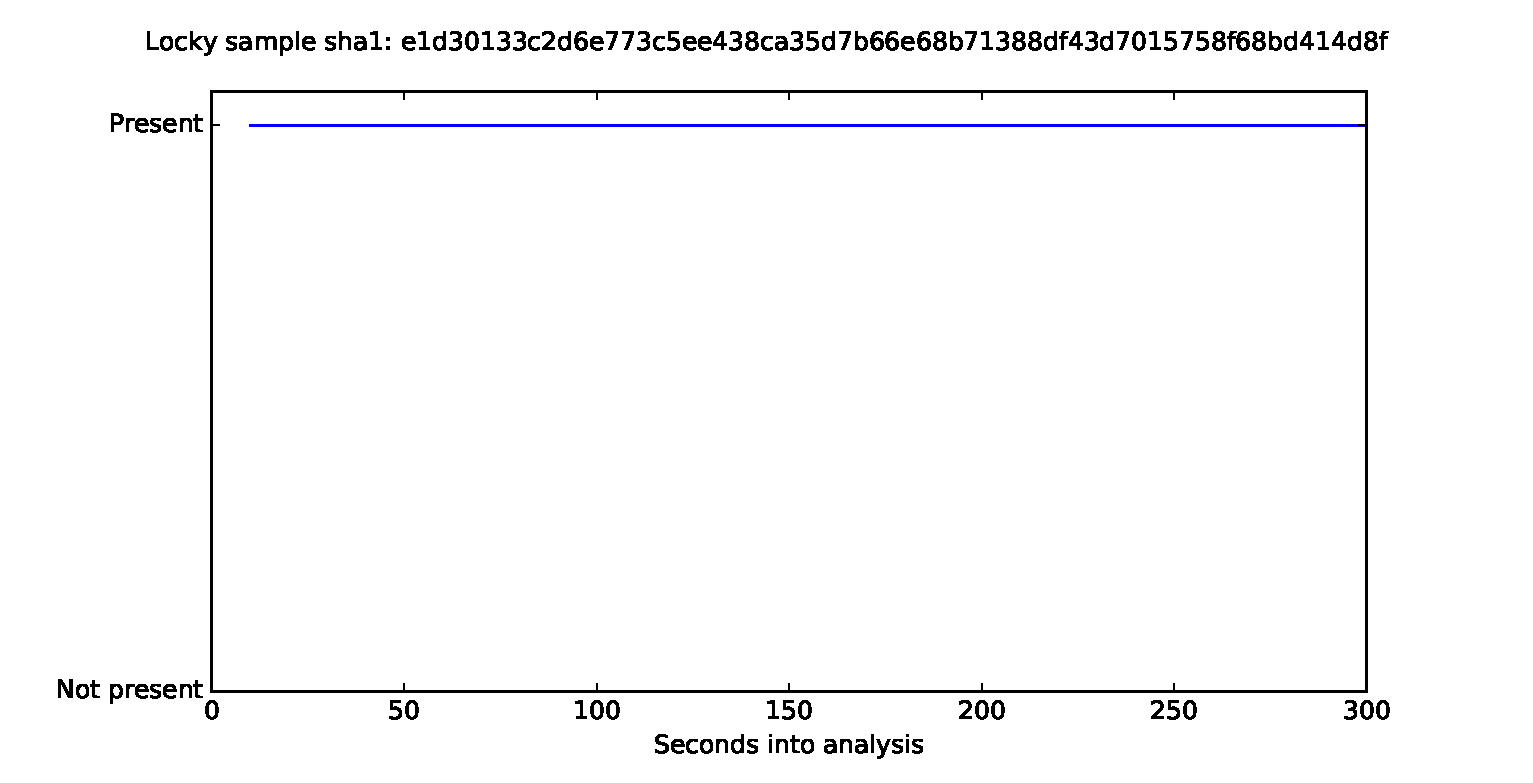
\includegraphics[width=8cm,scale=0.5]{images/locky/locky-timelines-eps/Locky-e1d30133c2d6e773c5ee438ca35d7b66e68b71388df43d7015758f68bd414d8f.eps}
    \caption{A Locky timeline showing the average of in-memory configuration data for an analysis in the 'Continuous communication' group}
    \label{fig:locky-timeline-continuous}
\end{figure}
\begin{figure}[!h]
    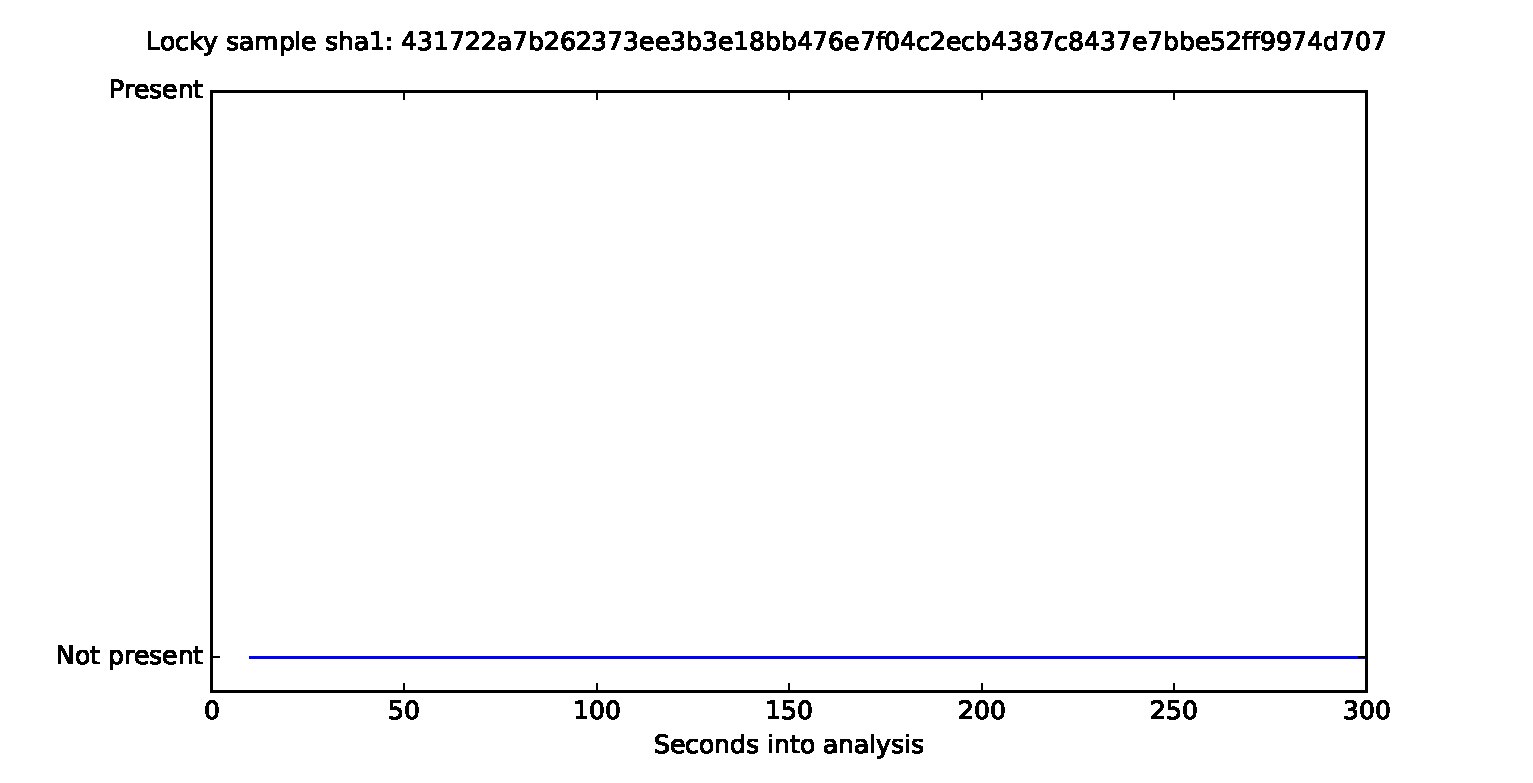
\includegraphics[width=8cm,scale=0.5]{images/locky/locky-timelines-eps/Locky-431722a7b262373ee3b3e18bb476e7f04c2ecb4387c8437e7bbe52ff9974d707.eps}
    \caption{A Locky timeline showing the average of in-memory configuration data for the 'Idle' group}
    \label{fig:locky-timeline-idle}
\end{figure}


\subsection{Results Teslacrypt}
The analysis of the Teslacrypt family resulted in data for 111 out of 115 used malware samples, four of the samples crashed upon execution. These samples are not part of any timelines or charts discussed in this subsection. Figure \ref{fig:teslacrypt-bar} shows the presence of configuration data for all measured Teslacrypt analyses. This chart was created by combining the timelines for all Teslacrypt analyses. All seperate timelines can be found at \footnote{\url{https://oege.ie.hva.nl/~zutpher003/research2016/teslacrypt/}}.


\begin{figure}[h]
	\hspace{-3cm}
    \includegraphics[width=13cm,trim=-70mm 0mm 0mm 9mm, clip=true]{images/teslacrypt/teslacrypt-barchart.eps}
    \caption{A chart showing the combined timelines of presence of configuration data during the analysis of all Teslacrypt samples}
    \label{fig:teslacrypt-bar}
\end{figure}

\textbf{Expected Teslacrypt behavior}\\
Analyses in this group display the 'expected' Teslacrypt behavior \cite{wyke-currans} and can be split into two types. The first type displays the following behavior. After execution, the first process starts by copying its binary and creating a process using this binary, which will be the actual malicious process. It differs per analysis how many times this copying occurs until the malicious binary is started, it happens one to four times. After the malicious process has started, the first binary is removed by starting a Windows command prompt and executing a delete command. The next step performed is the encryption of the user's files. When the encryption has finished, the malicious process attempts to communicate with its C2 and after this step create files which inform the user that their files have been encrypted.\\
\\The second group displays the similar behavior, but with the difference of first delaying execution by constantly reading the same registry key before starting the malicious process. This does result in two different timelines. With the first type, configuration data can be found almost the entire execution of the malware. With the second type only after it is done delaying execution, which takes an average of 60 seconds. A timeline for the first type can be seen at figure \ref{fig:teslacrypt-expected} and a timeline for the second type can be seen at figure \ref{fig:teslacrypt-expected-delay}.


\begin{figure}[!h]
    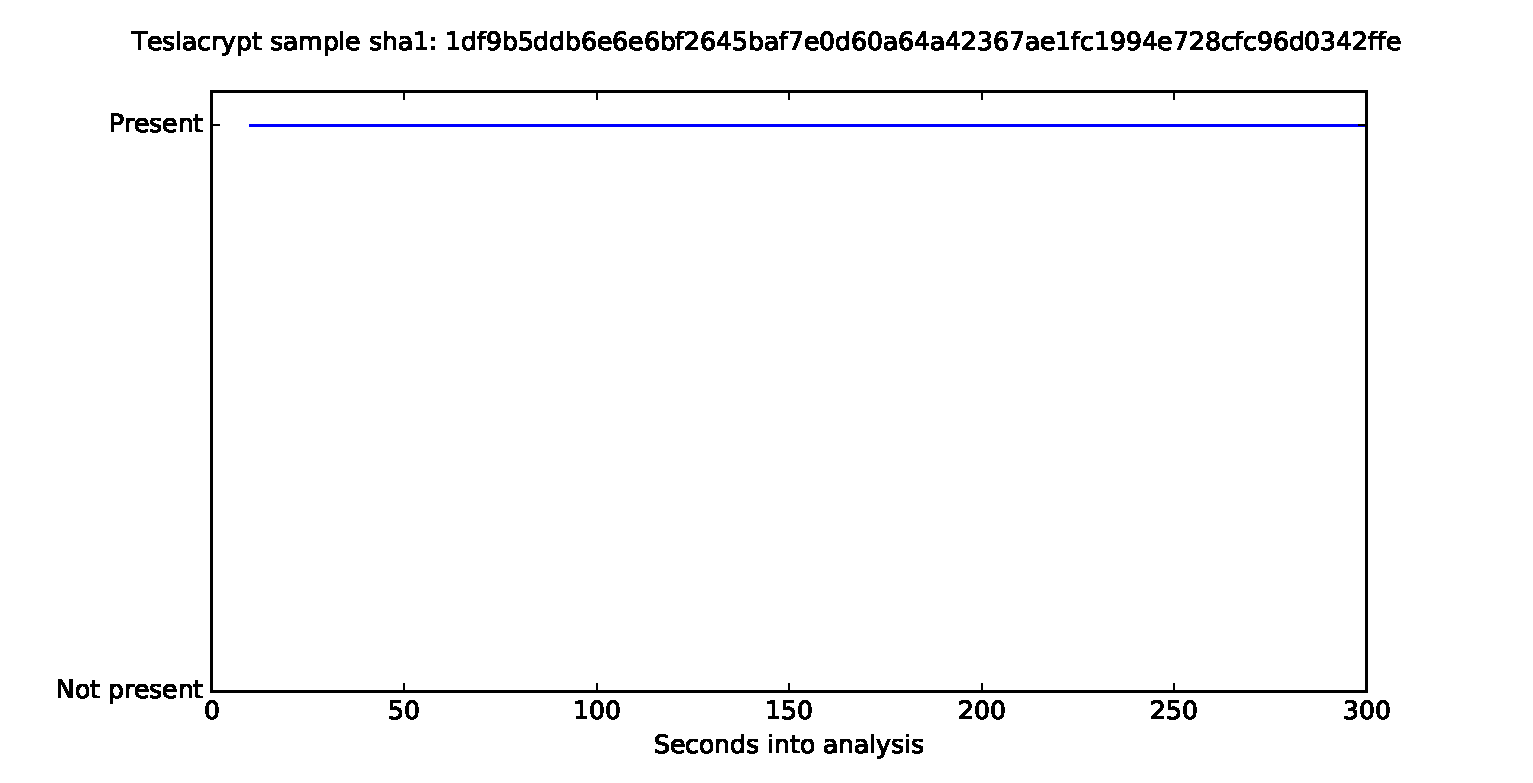
\includegraphics[width=8cm,scale=0.5]{images/teslacrypt/teslacrypt-timelines-eps/Teslacrypt-1df9b5ddb6e6e6bf2645baf7e0d60a64a42367ae1fc1994e728cfc96d0342ffe.eps}
    \caption{A Teslacrypt timeline showing the average of in-memory configuration data for an analysis in the 'Expected behavior' group}
    \label{fig:teslacrypt-expected}
\end{figure}
\begin{figure}[!h]
    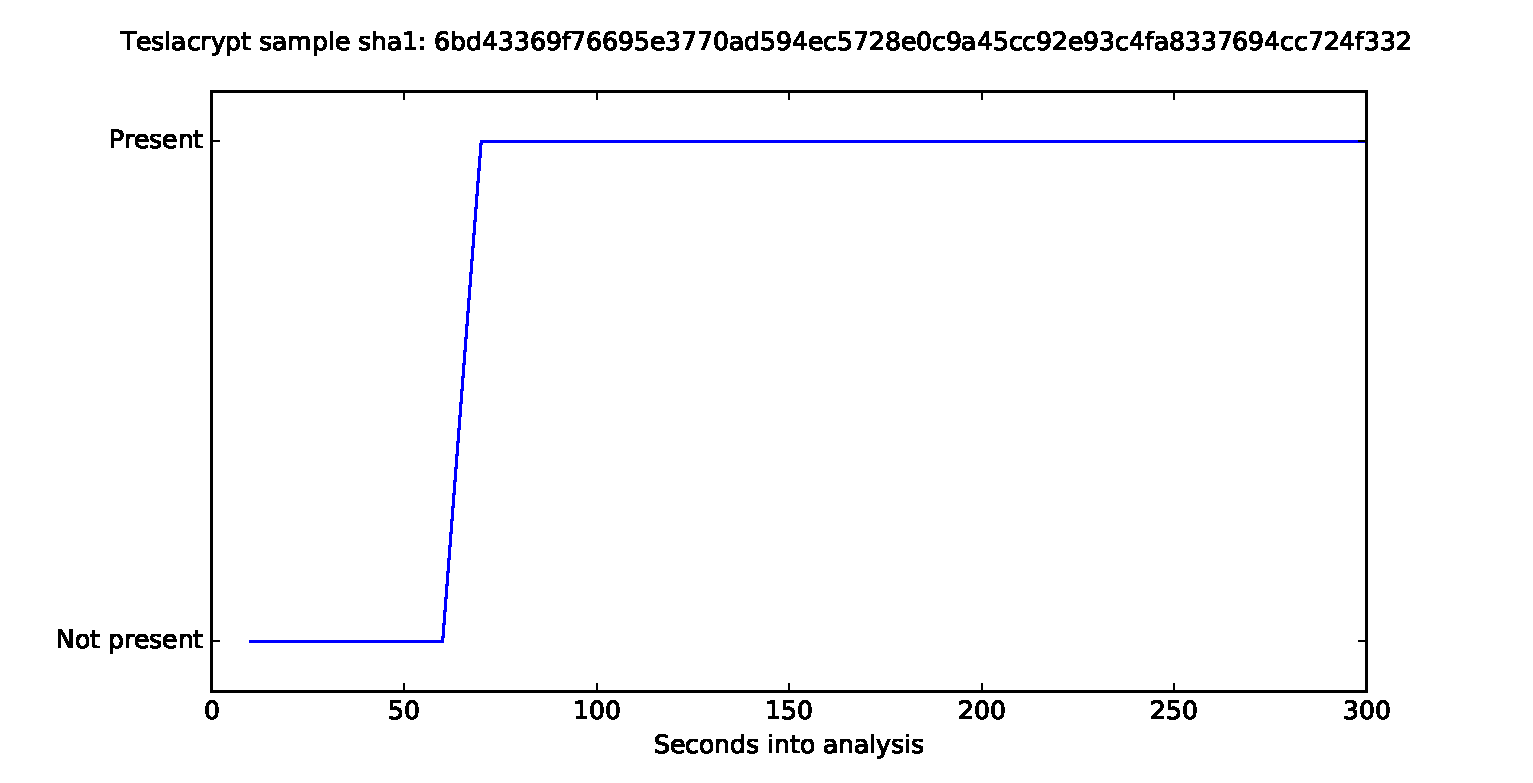
\includegraphics[width=8cm,scale=0.5]{images/teslacrypt/teslacrypt-timelines-eps/Teslacrypt-6bd43369f76695e3770ad594ec5728e0c9a45cc92e93c4fa8337694cc724f332.eps}
    \caption{A Teslacrypt timeline showing the average of in-memory configuration data for an analysis in the 'Expected behavior with execution delay' group}
    \label{fig:teslacrypt-expected-delay}
\end{figure}

\newpage
\subsection{Explanation of the observed behavior}
This subsection explains why some behavior was found. Mind that these are only hypotheses. Further research in these malware samples is needed to draw a proper conclusion about why this behavior occurs. Only behavior not following the expected behavior, which is described in the paper that is referenced in each malware group's 'Expected behavior' description, is included in this subsection.\\

\textbf{Delaying execution (sleeping)}\\
At least one group of all analysed malware families shows behavior that delays te execution. This was observed in two different forms: using the actual 'NtDelayExecution' or an equivalent Windows API call and using the same or a series of the same Windows API call which ends up delaying the execution because it is used hundreds of times in a row. \\A possible reason for observing these two types is that malware authors are aware of a simple 'NtDelayExectuion' call easily being recognized and countered by an automated malware analysis system. An example of this would be opening, reading and closing the same registry key over and over. \\\\It is likely that this action is performed as a form of automated dynamic malware analysis evasion or sandbox evasion. Usually, an automated analysis only runs for several minutes in which it collects all kinds of data. If no data that indicates malicious actions is collected, a malware sample might be labeled as non-malicious. Delaying the execution can be a means to reach this goal \cite{keragala-evasion}.\\

\textbf{Variation in the amount of binaries unpacked/copied}\\
All analysed malware families start by copying their own or unpacking a new binary to another location and starting it as the first action after execution. This copying and executing is likely done to make it harder to detect and remove the malware. The original binary is often removed after the second process has started. The amount copying and execution actions differs per malware and also within a malware family. A possible reason for this is that the dataset used for this research contains multiple versions of a certain malware family.\\

\textbf{No action, idle or brief behavior}\\
Nearly all analysed families have an 'Idle' group. This group contains analyses which either did perform any expected actions or delayed execution during the entire analysis. Multiple explanations for this behavior exist. Some malware is configured speficically for a target or a group of targets. An example being: Windows 7 users with an English system languange. It is possible that the 'idle' samples were configured for a target and that the analysis virtual machine did not meet the requirements to be in that target group.\\\\
A second reason for 'idle' behavior can be that the malware detects that it is being executed inside a sandbox, and Cuckoo Sandbox does not mitigate the method this malware uses to detect it. The malware might do this by looking for known names for virtual devices like network interfaces, hard drives and others. Other ways of detecting a sandbox are possible \cite{keragala-evasion}.\\

\textbf{Process/DLL injection}\\
Both banking malware families display the use of process/DLL injection. Specifically the type 'remote thread injection'. The malicious process opens a process handle which it uses to write a path of a malicious DLL to the process handle's memory. The malicious process then starts a remote thread using the 'CreateRemoteThread' API call which then loads the malicious DLL. This action is usually performed using a legitimate Windows process like Explorer.exe  \cite{alasiri-dll-injection}.\\\\There are multiple likely reasons a malware author chose to use this. The first reason is that is allows for the first process to exit and the malware run under a legitimate Windows process name. The second reason is that a legitimate process is likely to keep running as long as the operating system is running. A third reason is that this allows for the malware to only exist in the system memory and not on disk, which makes it harder to detect.\\

\textbf{Crashed}\\
Some of the malware families also contain a 'Failed or crashed' group. The malware process in the analyses of this group crashed. There are several reasons for this, the two most observed reasons are: trying to access a part of the memory to which the malware process does not have access and it being killed as a result. The second reason observed is the importing of non-existing DLLs, which also results in crashes.

% trigger a \newpage just before the given reference
% number - used to balance the columns on the last page
% adjust value as needed - may need to be readjusted if
% the document is modified later
%\IEEEtriggeratref{8}
% The "triggered" command can be changed if desired:
%\IEEEtriggercmd{\enlargethispage{-5in}}

% references section

% can use a bibliography generated by BibTeX as a .bbl file
% BibTeX documentation can be easily obtained at:
% http://mirror.ctan.org/biblio/bibtex/contrib/doc/
% The IEEEtran BibTeX style support page is at:
% http://www.michaelshell.org/tex/ieeetran/bibtex/
%\bibliographystyle{IEEEtran}
% argument is your BibTeX string definitions and bibliography database(s)
%\bibliography{IEEEabrv,../bib/paper}
%
% <OR> manually copy in the resultant .bbl file
% set second argument of \begin to the number of references
% (used to reserve space for the reference number labels box)

\afterpage{\blankpage}
\newpage
\apptocmd{\thebibliography}{\setlength{\itemsep}{3pt}}{}{}
\begin{thebibliography}{}

\bibitem{tran-cryptolocker}
M. tran, "CryptoLocker and the Rise of Cryptographic Ransomware",
Tufts University, 2014.

\bibitem{wyke-currans}
J. Wyke and A. Ajjan , "The Current State of Ransomware",
Sophos, 2015, pp. 36-42.

\bibitem{long-locky}
J. Long, "Locky: The New Face of Ransomware",
East Carolina University, 2016.

\bibitem{brien-dridex}
D. O'Brien, "Dridex: Tidal waves of spam pushing dangerous financial Trojan",
Symantec, 2016, pp. 21-24.

\bibitem{wyke-zeus}
J. Wyke, "What is Zeus"
Sophos, 2011, pp. 10-13.

\bibitem{kroustek-vawtrak}
J. Křoustek, "Analysis of Banking Trojan Vawtrak", 
AVG Technologies, Virus Lab, 2015, pp. 10-11.

\bibitem{wyke-confextract}
J. Wyke, "Breaking the bank(er): Automated configuration data extraction for banking malware", 
Sophos, 2015, pp. 5,9.

\bibitem{cuckoo}
https://cuckoosandbox.org/.

\bibitem{teller-memory}
T. Teller and A. Hayon, "Enhancing Automated Malware Analysis Machines with Memory Analysis",
2014, pp. 1-2.

\bibitem{vmcloak}
http://vmcloak.org/

\bibitem{roberston-ioc}
C. Roberston, "Indicators of compromise in memory forensics,"
SANS, February 2013. 

\bibitem{hamrock-entropy}
J. Hamrock and R. Lyda, "Using Entropy Analysis to Find Encrypted and Packed Malware", IEEE Computer Society, 2007, pp. 1-3.

\bibitem{sahin-vawtrak}
E. Sahin and J. Wyke, "Vawtrak v2",
Sophos, 2016, pp. 34-42.

\bibitem{nelson-locky}
P. Nelson, "Locky Ransomware Analysis",
https://www.sternsecurity.com/blog/locky-ransomware-analysis
Stern Security, 2015.

\bibitem{zeus-ioc}
Sourcefire Vulnerability Research Team, "Zeus Trojan Analysis"
https://labs.snort.org/papers/zeus.html
Sourcefire

\bibitem{vawtrak-ioc}
D. Huss and M. Mesa, "In the Shadows: Vawtrak Aims to Get Stealthier by adding New Data Cloaking",
https://www.proofpoint.com/us/threat-insight/post/In-The-Shadows
Proofpoint, 2015

\bibitem{keragala-evasion}
D.  Keragala, "Detecting Malware and Sandbox Evasion Techniques",
SANS, January 2016, pp. 2-6

\bibitem{alasiri-dll-injection}
A. Alasiri, M. Alzaidi , D. Lindskog, P. Zavarsky, R. Ruhl, S. Alassmi,
"Comparative Analysis of Operational Malware Dynamic Link",
Concordia University College of Alberta, July 2012,
pp. 1-5.

\end{thebibliography}


\afterpage{\blankpage}
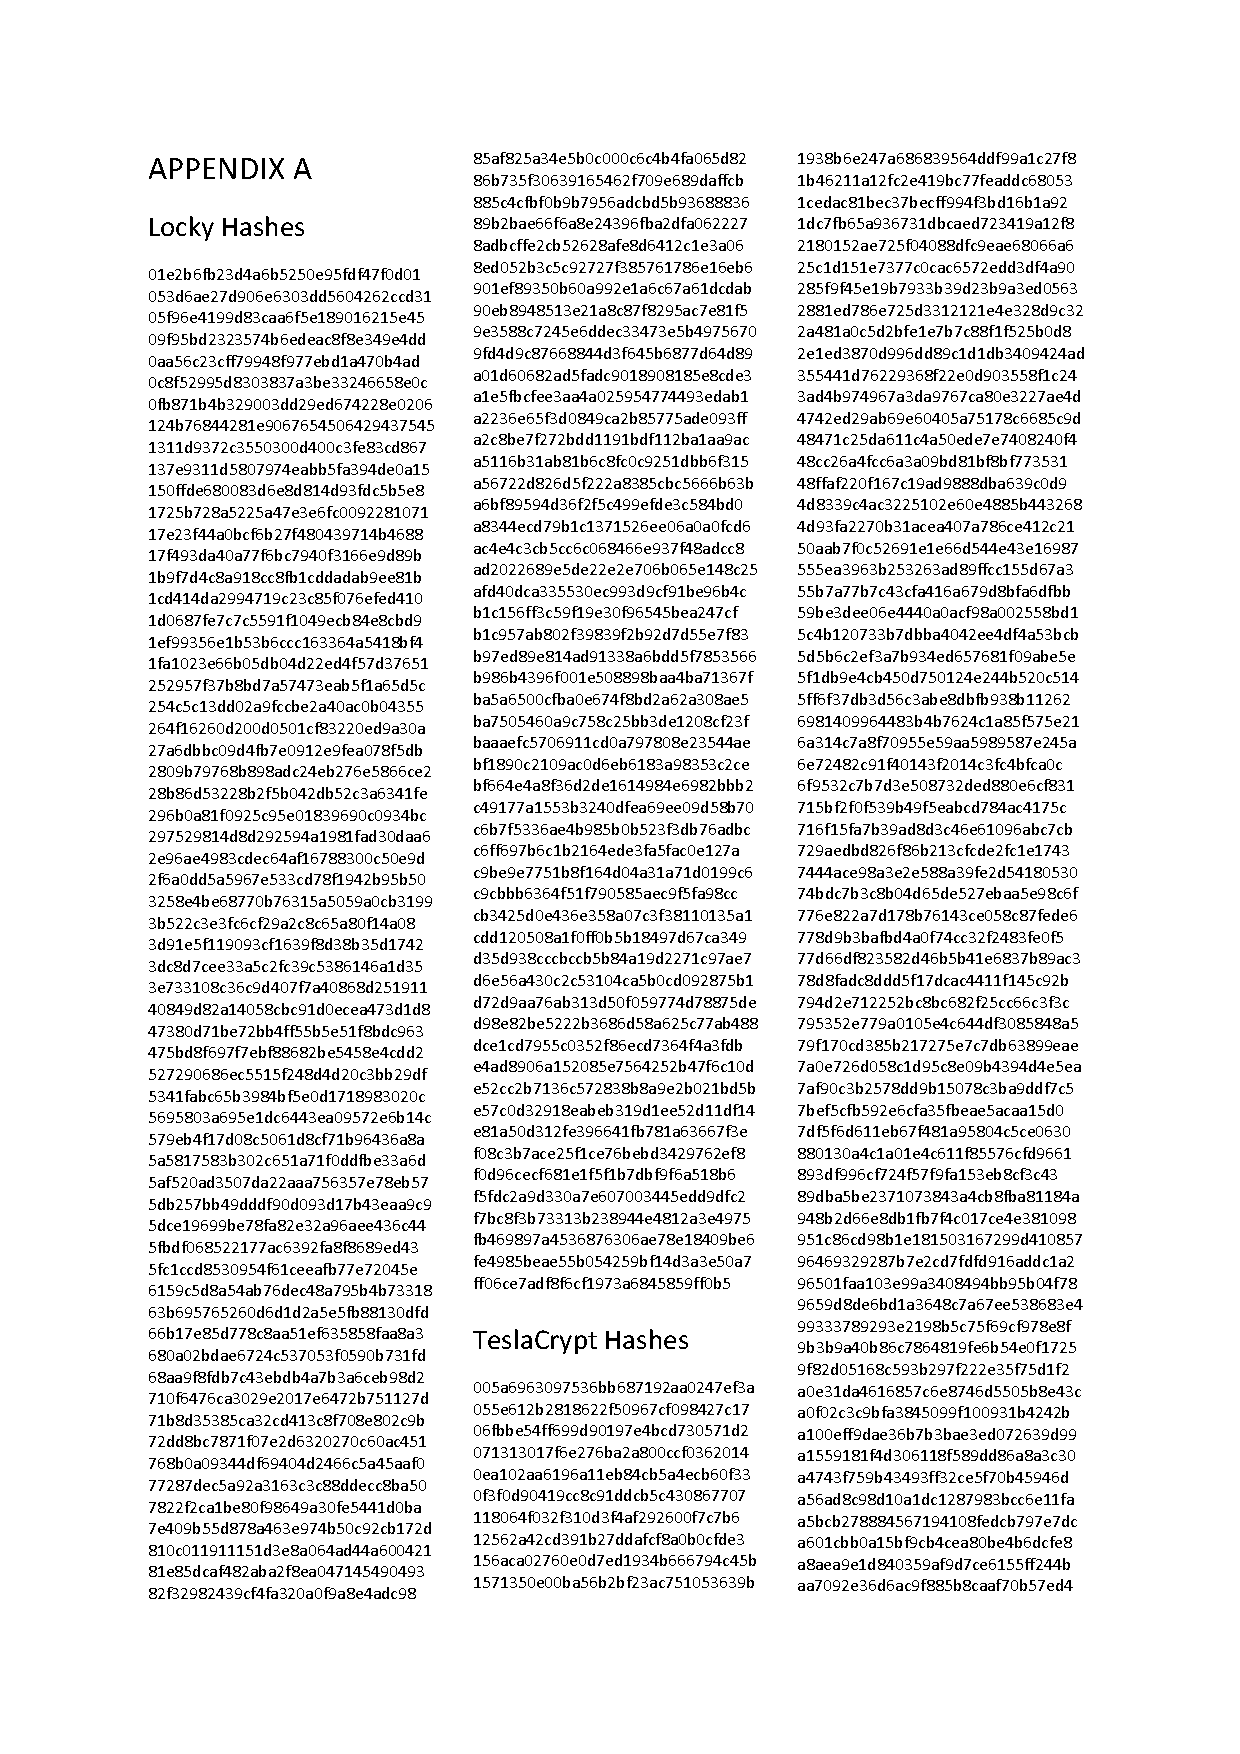
\includepdf[pages={1-3}]{appendices/Appendix-A-hashes.pdf}
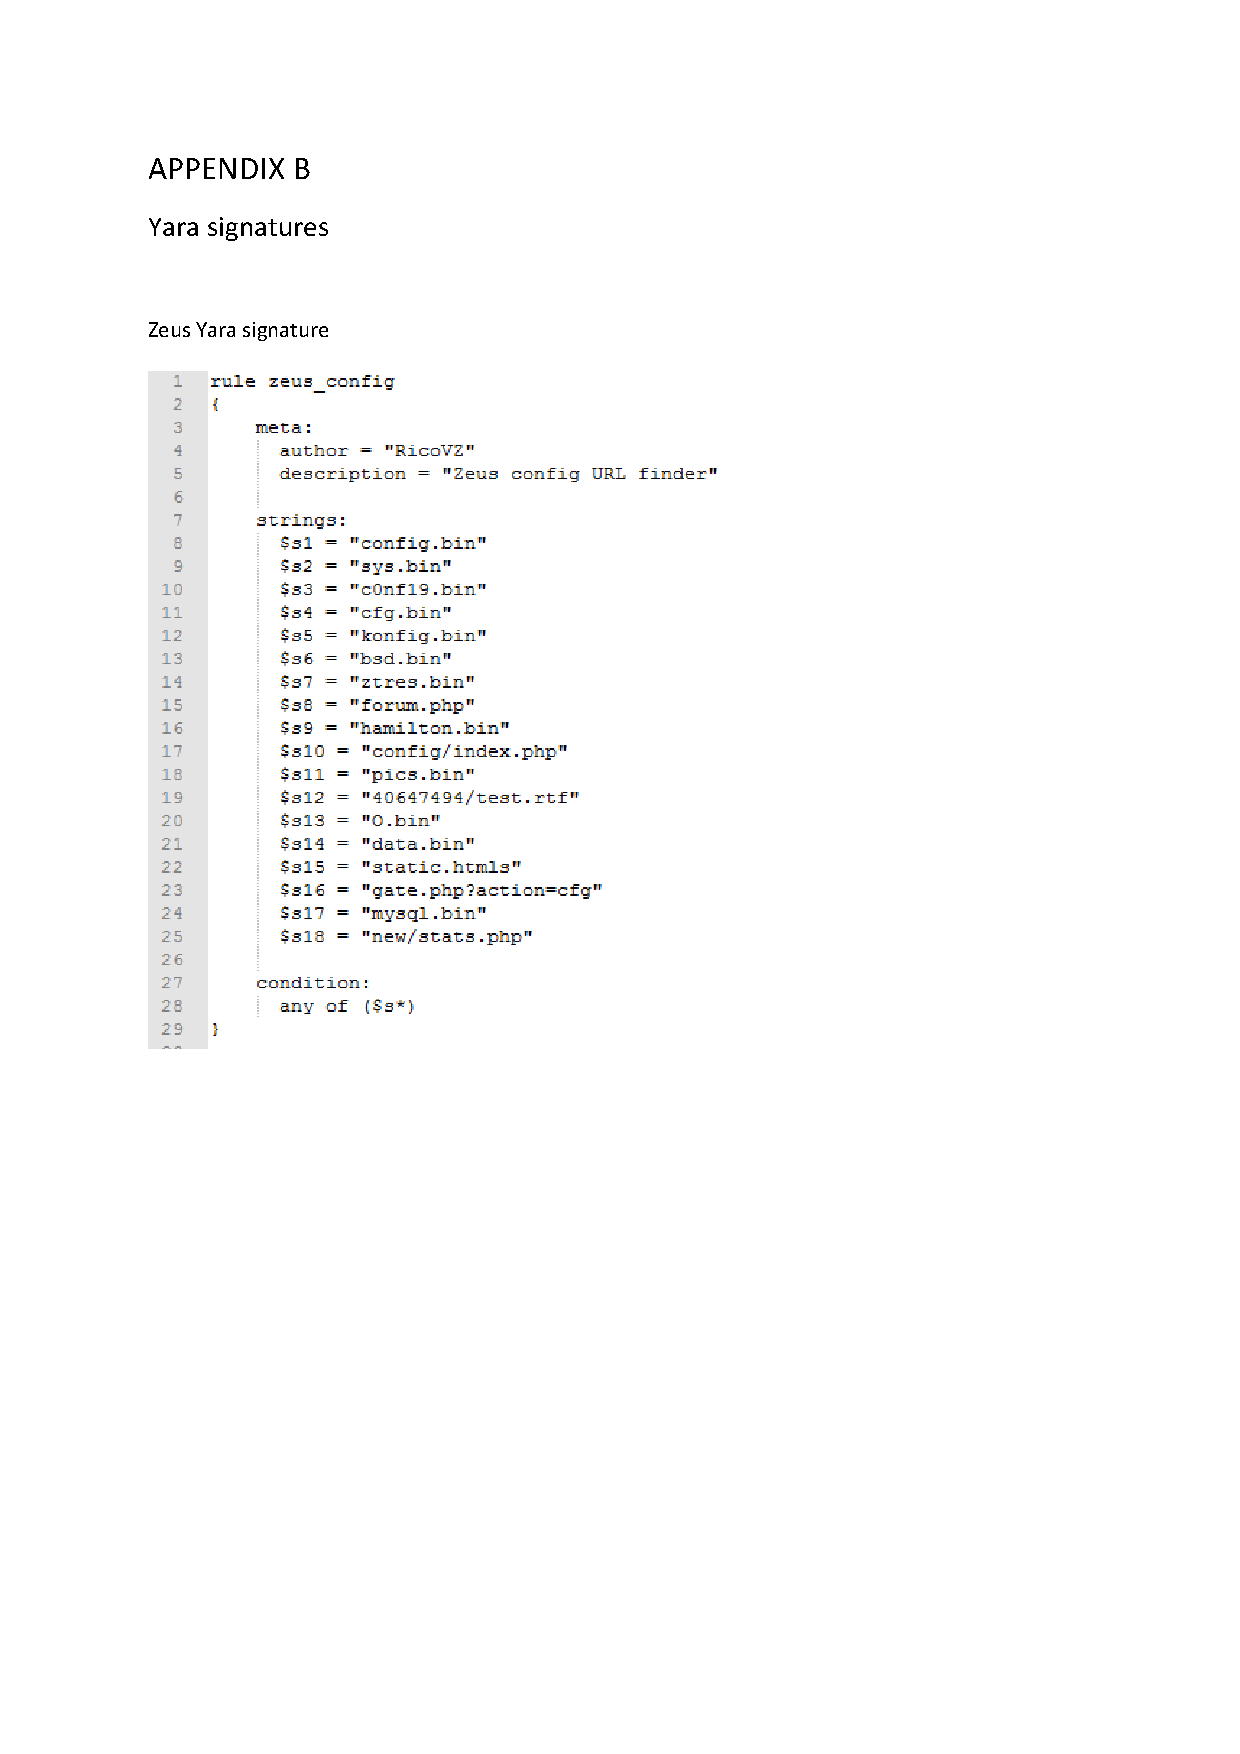
\includepdf[pages={1-4}]{appendices/Appendix-B-signatures.pdf}


\end{document}


